\documentclass[hyperref, plainreport, noproblem]{cgvpub1}

\usepackage{color}
\usepackage{graphicx}

\usepackage{amsmath}


\usepackage{amssymb}
\usepackage{amsthm}
\usepackage{mathtools}
\usepackage{float}
\usepackage{tikz}
\usepackage{epstopdf}
%\usepackage{natbib}
\usepackage{hyperref}
\usepackage{multirow}

\usepackage[left=2.5cm, right=2.5cm, top=3cm, bottom=3.5cm]{geometry}

\usepackage{caption}
\usepackage{subcaption}

\graphicspath{ {figures/} }

\newtheorem{theorem}{Theorem}
\newtheorem{lemma}{Lemma}

\newcommand{\myeq}{=}
\newcommand{\expc}[1]{\mathrm{E} \! \left[#1\right]}
\newcommand{\re}[1]{\mathrm{Re}\! \left(#1\right)}
\newcommand{\im}[1]{\mathrm{Im}\! \left(#1\right)}
\newcommand{\prob}[1]{\mathrm{Pr}\! \left(#1\right)}
\newcommand{\probC}[1]{\mathrm{Pr}_\epsilon\! \left(#1\right)}

\newcommand{\comment}[1]{{\color{red}[\textit{#1}]}}

%\newcommand{\comment}[1]{}

\newcommand{\eqn}[1]{(\ref{#1})}

\newcommand{\fig}[1]{Fig.~\ref{#1}}

%\newcommand{\doc}[1]{{\tiny #1}}
\newcommand{\doc}[1]{}

\newcommand{\tikzfolder}{./tikz-files/}

\input{\tikzfolder tikz-styles}

%\usepackage{draftwatermark}
%\SetWatermarkText{DRAFT}
%\SetWatermarkScale{0.5}



\author{alaleh}
\title{The title of the thesis}
\birthday{1. Januar 1234}
\placeofbirth{Dresden}
\matno{123456, 123}
\betreuer{Dr. B. Spline}
%\bibfiles{literature-example}
%\problem{Write down your task...}
\copyrighterklaerung{If the author used resources from third parties (texts, images, code) he or she should state the consents of the copyright owners here or cite the given general conditions (e.g. CC/(L)GPL/BSD copyright notices)}


\begin{document}


\chapter{Introduction}

Tractography is a kind of scientific visualization technique used to visualize the nerve tract data. The data we use here is diffusion magnetic resonance imaging(DMRI). To show the 3D DMRI brain data we basically use two kinds of colormaps. The first scalar colormap is to compute the scalar values such as fractional anisotropy which represent the characteristics of diffusion and map it to the tracts. The second one is to use spherical colormaps to present orientation of tracts. After implementation we will compare the advantages and disadvantages of these colormaps and do the evaluation.

The aim of the project is to implement the visualization of tractography. The goals include: (1)Literature review on real-time tube rendering with color mapping specific to tractography data. (2) Study and implementation of ensemble scalar and orientation colormaps to visualize fiber tracts. (3) Study and implementation of ensemble comparison and localization based on the chosen colormaps. (4) Selection of viewpoints to conduct robust visualization of DMRI fiber tube characteristics. (5) Evaluation of the ensemble colormaps for accuracy and effectiveness of tract visualization effects. (6) Study of transparency effects to better visualize the eloquent crossing fiber tracts (optional).

In this project, we implement the scalar color mapping and spherical color mapping. The scalar colormaps include coolwarm, extended Kindlmann, isoluminant rainbow, black body and extended black body. We map the fractional anisotropy (FA) and mean diffusivity(MD) value to the tract positions. Besides, we also implement the spherical colormaps of absolute value method and boy’s surface method. To compare the colormaps we evaluate the effects of different colormaps and draw some conclusions.

The report includes several parts as below: the literature review on related work, basic knowledge about this project, the process of implementation and evaluation.


\chapter{Ralated work}


\subsubsection*{Coolwarm colormap}
Coolwarm colormap is a diverging colormap mentioned by Kenneth Moreland. It is double-ended, monotonic on each side, with smooth transition in the middle.

\subsubsection*{Kindlmann colormap}
Kindlmann colormap was introduced by Gordon Kindlmann, which samples the standard rainbow colors (going from magenta through blue and green to red), and matching against lightness increasing linearly from 0.0 to 1.0, \cite{kindlmann} making it much more perceptually viable. Extended Kindlmann colormap uses the colors from Kindlmann, but also adding more hues.

\subsubsection*{Blackbody colormap and extended blackbody colormap}
K. Moreland mentioned in his paper \cite{moreland2016} that the disadvantages of rainbow colormap in the area of visualization. Among them, he applied pseudocoloring on the 2D scalar field. In order to reduce the problem of color map contrast, he proposed two examples, blackbody and extended blackbody colormap. The blackbody colormap is based on the radiation of blackbody. It is inspired by the color of light emitted by objects kept at different temperatures. The color distribution is modified to pursue linear perception. The extended blackbody adds purple and blue hues to the blackbody colormap to improve the inconsistency of the yellow-white transition. 

\subsubsection*{Isoluminant rainbow colormap}
Isoluminant rainbow is a multihued colormap where the luminance is equal. Isoluminant colormaps are invariant in contrast of lightness. In Kindlmann’s work, an isoluminant rainbow colormap is generated. There are 6 color points: red, yellow, green, cyan, blue and magenta which represented by RGB value and they are evenly spaced \cite{kindlmann}. Isoluminant rainbow colormap is poor at showing quantitative characteristics because it is not perceived ordered \cite{moreland2019}. 

\section{Spherical colormaps}

In spherical color mapping, the colors on the sphere can be used to represent the orientation. In this project we focus on two spherical color maps: absolute colormap and Boy’s surface colormap.


\subsubsection*{Absolute value}
Pajevic and Pierpaoli use the absolute value method to solve the symmetry issues \cite{pajevic}. In absolute colormap, it is mirror and rotational symmetric at the same time. The unit value of the eigenvectors will be directly mapped to the RGB values of the colors. The sign of the eigenvector does not affect the results and only the absolute values will be considered. The advantage of this colormap is that it can show the direction change in all dimensions in 3D. Absolute colormap is a good choice for default spherical colormap \cite{moreland2019}.

\subsubsection*{Boy’s Surface}  
To be done…

\section{Measuring methods}
In the study conducted by Chen et al, they tested six ensemble scalar color maps for fractional anisotropy and four spherical colormaps for ensemble orientation of tracts. The evaluation process is explicitly given and they also discuss the results of different visualizations. There are four types of tasks: ensemble identification, ensemble localization, ensemble comparison and ensemble association. In conclusion, the scalar color maps of blackbody, extended blackbody and coolwarm are the best choices to present the ensemble average. The number of hues have more impacts than the luminance. Spherical colormaps such as absolute and Boy’s surface can show the ensemble orientation of tracts better than the other ones \cite{moreland2019}. The evaluation methods in our project are inspired by the study.

\chapter{Basics}

\section{Tractography}
Tractography is a method to visualize the brain fiber tracts, which utilizes the directional diffusion in voxels. It is a tool to visualize white matter trajectories in vivo and noninvasively, so that we can study the human brain anatomy, such as brain connectivity.

Tractography visualization is built on the Diffusion Magnetic Resonance Imaging (dMRI) data, which is analyzed from the diffusion of free water in the brain. The diffusion of free water is termed as isotropic and it becomes anisotropic when there are barriers. 

\begin{figure}[h]
	\centering
	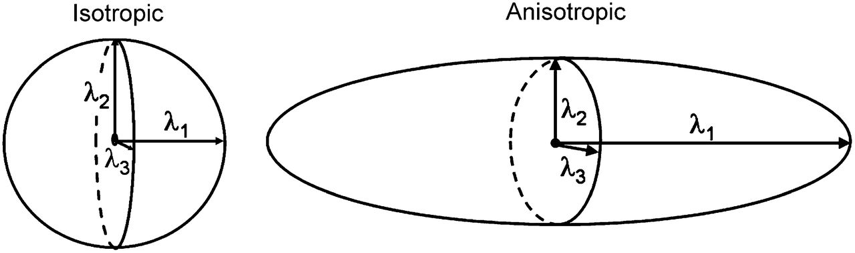
\includegraphics[width=0.7\textwidth]{iso_ani_diff}
	\caption{Isotropic and anisotropic diffusion with  being eigenvalues. From
https://neoreviews.aappublications.org/content/14/10/e483/tab-figures-data \comment{biblio}}
	\label{fig:iso_ani_diff}
\end{figure}

The diffusion in brain is anisotropic so it is represented as an ellipsoid as in the right figure in Figure~\ref{fig:iso_ani_diff}. The three eigenvalues  $\lambda_1, \lambda_2, \lambda_3$ represent the three axes of the ellipsoid. The vector associated with the latest eigenvalue is assumed as the local fiber direction.\cite{tak}
Using dMRI, the apparent diffusion coefficient at each voxel of the image can be calculated and the whole diffusion tensor can be constructed by multilinear regression across multiple images.

\section{Fractional Anisotropy and Mean Diffusivity }
One way to measure the anisotropic diffusion is fractional anisotropy (FA), which is a scalar ratio from 0 to 1, with 0 representing isotropic and 1 as an ideal linear diffusion. It represents the degree of alignment of cellular structures within fiber tracts and their structural integrity \cite{cer}.

Another often used measurement is mean diffusivity (MD), which describes the average mobility of water molecules. It is equal to one third of the trace of the diffusion tensor. MD is affected by cellular size and integrity and independent of any tissue directionality. \cite{cer}

Here is the formula of FA and MD $\lambda_1, \lambda_2, \lambda_3$  are Eigenvalues of the diffusion tensor.

\begin{equation}
	FA=\sqrt{\frac{3 \sum_{i=1}^{3}(\lambda_i-\bar{l\lambda})^2}{2\sum_{i=1}^3\lambda_i^2}}, \quad FA\text{ in } [0,1]
\end{equation}

\begin{equation}
	MD=\frac{D_{xx}+D_{yy}+D_{zz}}{3}= \frac{\lambda_1+\lambda_2+\lambda_3}{3}
\end{equation}

\section{ Color mapping interpolation }
With the known discrete voxel FA/MD value, a simple linear interpolation method is used to construct new data points in between, thus obtaining a fiber track with continuous colormapping.

\begin{table}[h]
\caption{coolwarm colormap example}
\centering
\begin{tabular}{|c|c|c|c|c|}
\hline
colormap bar     & FA value & RGB\_r & RGB\_g & RGB\_b   \\ \hline
\multirow{8}{*}{
\includegraphics{coolwarm_bar} } & 0.0      & 85     & 72     & 193      \\ [5pt] \cline{2-5}
	& 0.1      & 125    & 135    & 239      \\ [6pt] \cline{2-5}
	& 0.3      & 166    & 185    & 255      \\ [6pt] \cline{2-5}
	& 0.4      & 205    & 215    & 240      \\ [6pt] \cline{2-5}
	& 0.6      & 235    & 209    & 194      \\ [6pt] \cline{2-5}
	& 0.7      & 243    & 168    & 137      \\ [6pt] \cline{2-5}
	& 0.9      & 222    & 106    & 83       \\ [6pt] \cline{2-5}
	& 1        & 177    & 1      & 39      \\ [6pt] \hline
\end{tabular}
\label{tbl:coolwarm}
\end{table}

Here is the linear interpolation formula:
\begin{equation}
 \frac{(y-y_0)}{(x-x_0)} = \frac{(y_1-y_0)}{(x_1-x_0)}
\end{equation}

\begin{figure}[h]
	\centering
	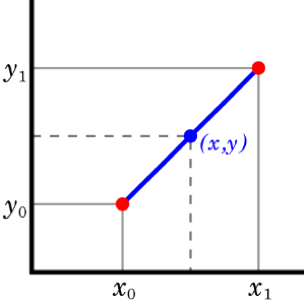
\includegraphics[width=0.4\textwidth]{interp}
	\caption{ linear interpolation 
Source: wiki \comment{biblio}}
	\label{fig:interp}
\end{figure}

\chapter{Implementation}

We use the CGV framework for task solutions implement. This framework is a set of highly coupled C++ libraries designed to use OpenGL to quickly develop prototypes of performance-intensive applications in the field of visualization and computer graphics research. It is very suitable for window and graphics context creation, event processing, GUI creation, interaction, and many common computer graphics algorithms and data structures required in our task.

\section{The colormap choosing and implement}
Generally, methods are defining a function or using numeric values to map to colors. This report defines the colormap by selecting colors that are continuously mapped to a series of values. 
There are two categories of color mapping methods:
\begin{itemize}
	\item Scalar Color Mapping: Consider a scalar value associated with each segment of a tract, which could  be FA or MD in this context. This type of color mappings provide a mapping from the chosen scalar quantity to a color. 
	\item Spherical Color Mapping: Unlike scalar color mapping, this type of mapping is usually from an inherent property of the tract segments to a color. A common choice is the orientation of the line segment. 
\end{itemize}

In this report, we examine 5 scalar and two spherical color mappings. 

\subsection*{Scalar colormappings}

These colormaps are recommended by Moreland et al., including: coolwarm, extended kindlmann, isoRainbow, black body, extended black body. The reason for choosing these pictures is that their popularity is relatively high. Figure~\ref{fig:1} shows those five different colormaps.

\begin{itemize}
	\item Coolwarm is a diverging color map (double ended) with a smooth transition in the middle. It is monotonic luminance and can avoid dark colors to allow shading. 

	\item Extended kindlmann uses the colors from kindlmann, but also adding more hues, which is perceptually viable with luminance change monotomically. 

	\item Blackbody is based on colors form black-body radiation. The luminance of it is perceptually linear, which can reinforce the imterpretation of the colors.

	\item Extended Blackbody is based on Blackbody colormap, adding some purple and blue hues. It is more appealing display and improve upon the narrow hue range of its red-yellow cousin than blackbody color map. 

	\item Isoluminant-rainbow is a multihues rainbow colormap, which the colors are more saturated.
\end{itemize}
\begin{figure}[ht]
    \centering
    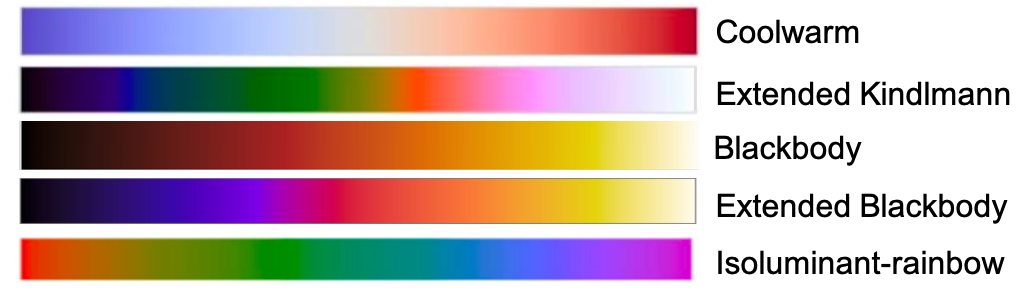
\includegraphics[width = 0.8\columnwidth]{1}
    \caption{ Five Scalar colosmaps.}
    \label{fig:1}
\end{figure}	

\subsection*{Spherical colormappings}
The spherical color mappings are
\begin{itemize}
	\item Absolute value method [cite] is a commonly used color mapping which maps the major axes, to major color components Red, Greed and Blue. The mapping is defined as 
	\begin{equation}
		f(\mathbf{s})=[|s_x|, \ |s_y|, \ |s_z|]^T
	\end{equation}
	where $\mathbf{s}=[s_x ,s_y, s_z]^T$ is the normalized vector corresponding to a line segment.  
	\begin{figure}
		\centering
		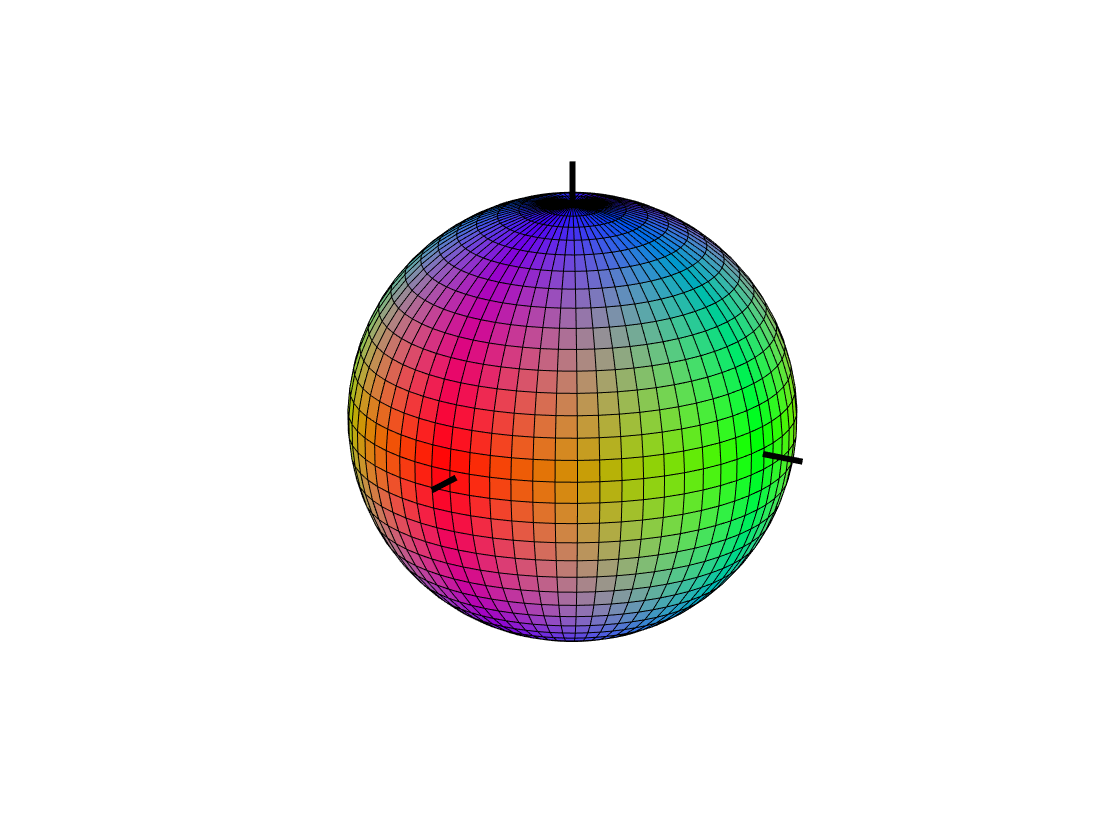
\includegraphics[width=0.35\textwidth]{absolute}
		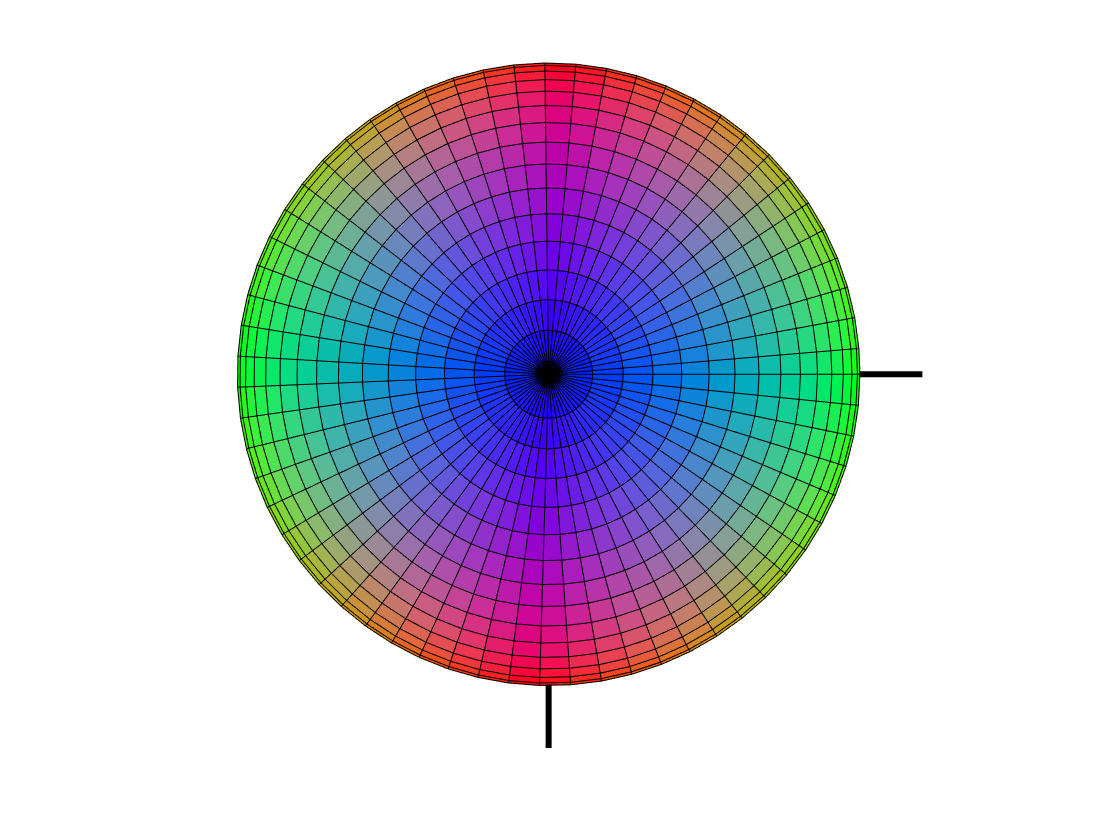
\includegraphics[width=0.3\textwidth]{absolute_top}
		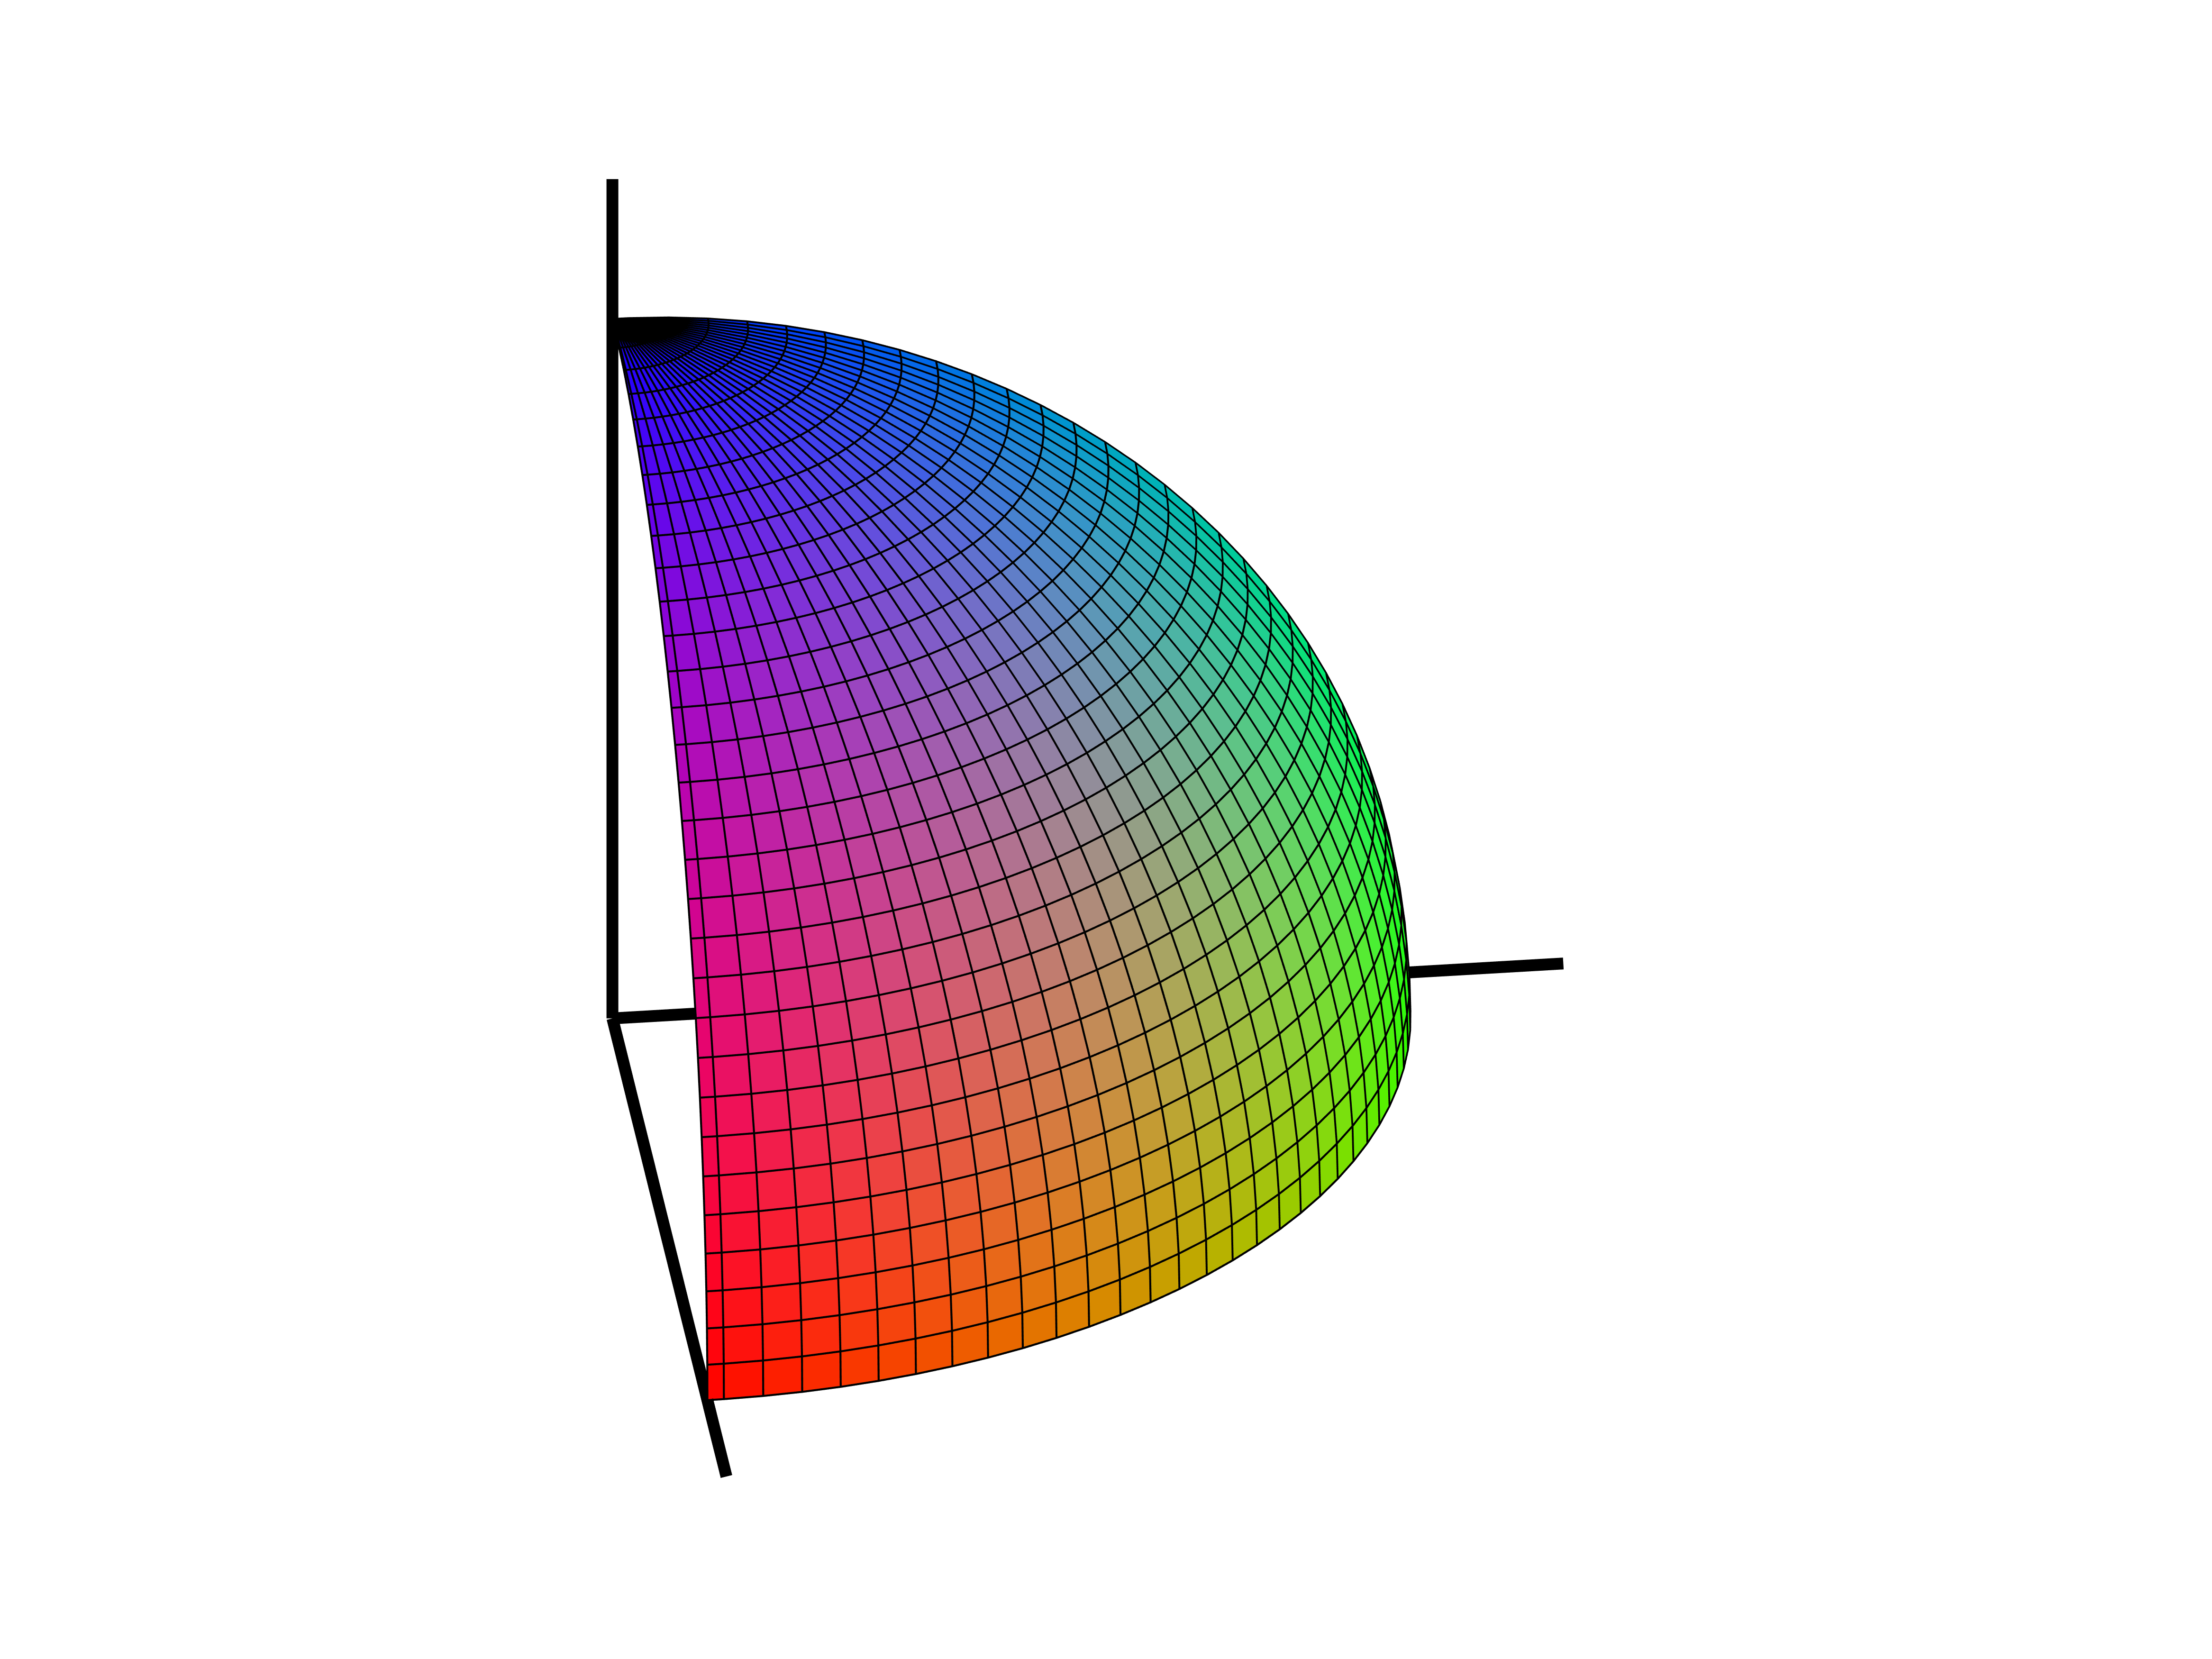
\includegraphics[width=0.3\textwidth]{absolute_octant}
		\caption{Absolute value method, colored sphere.}
	\end{figure}
	
	\item Boy's surface method is a more complicated color mapping scheme based on the immersion of Real Projective Plane in $\mathbb{R}^2$. The mapping is defined as 
	\begin{equation}
		f(\mathbf{s})=[f_1(\mathbf{s}), f_2(\mathbf{s}), f_3(\mathbf{s})]^T
	\end{equation}
	where 
	\begin{equation}
		f_i(\mathbf{s})=\sum_{j=0}^{\infty} c_{i,j} h_j(\mathbf{s}).
	\end{equation}
	
The functions $h_j$ are the spherical harmonics, a similar concept to harmonics in Fourier analysis. As suggested by the authors in [cite], the summation is replaced with a partial sum to obtain a continuous mapping and the coefficients $c_{i,j}$ are adjusted manually for better results. 
\end{itemize}

	\begin{figure}
		\centering
		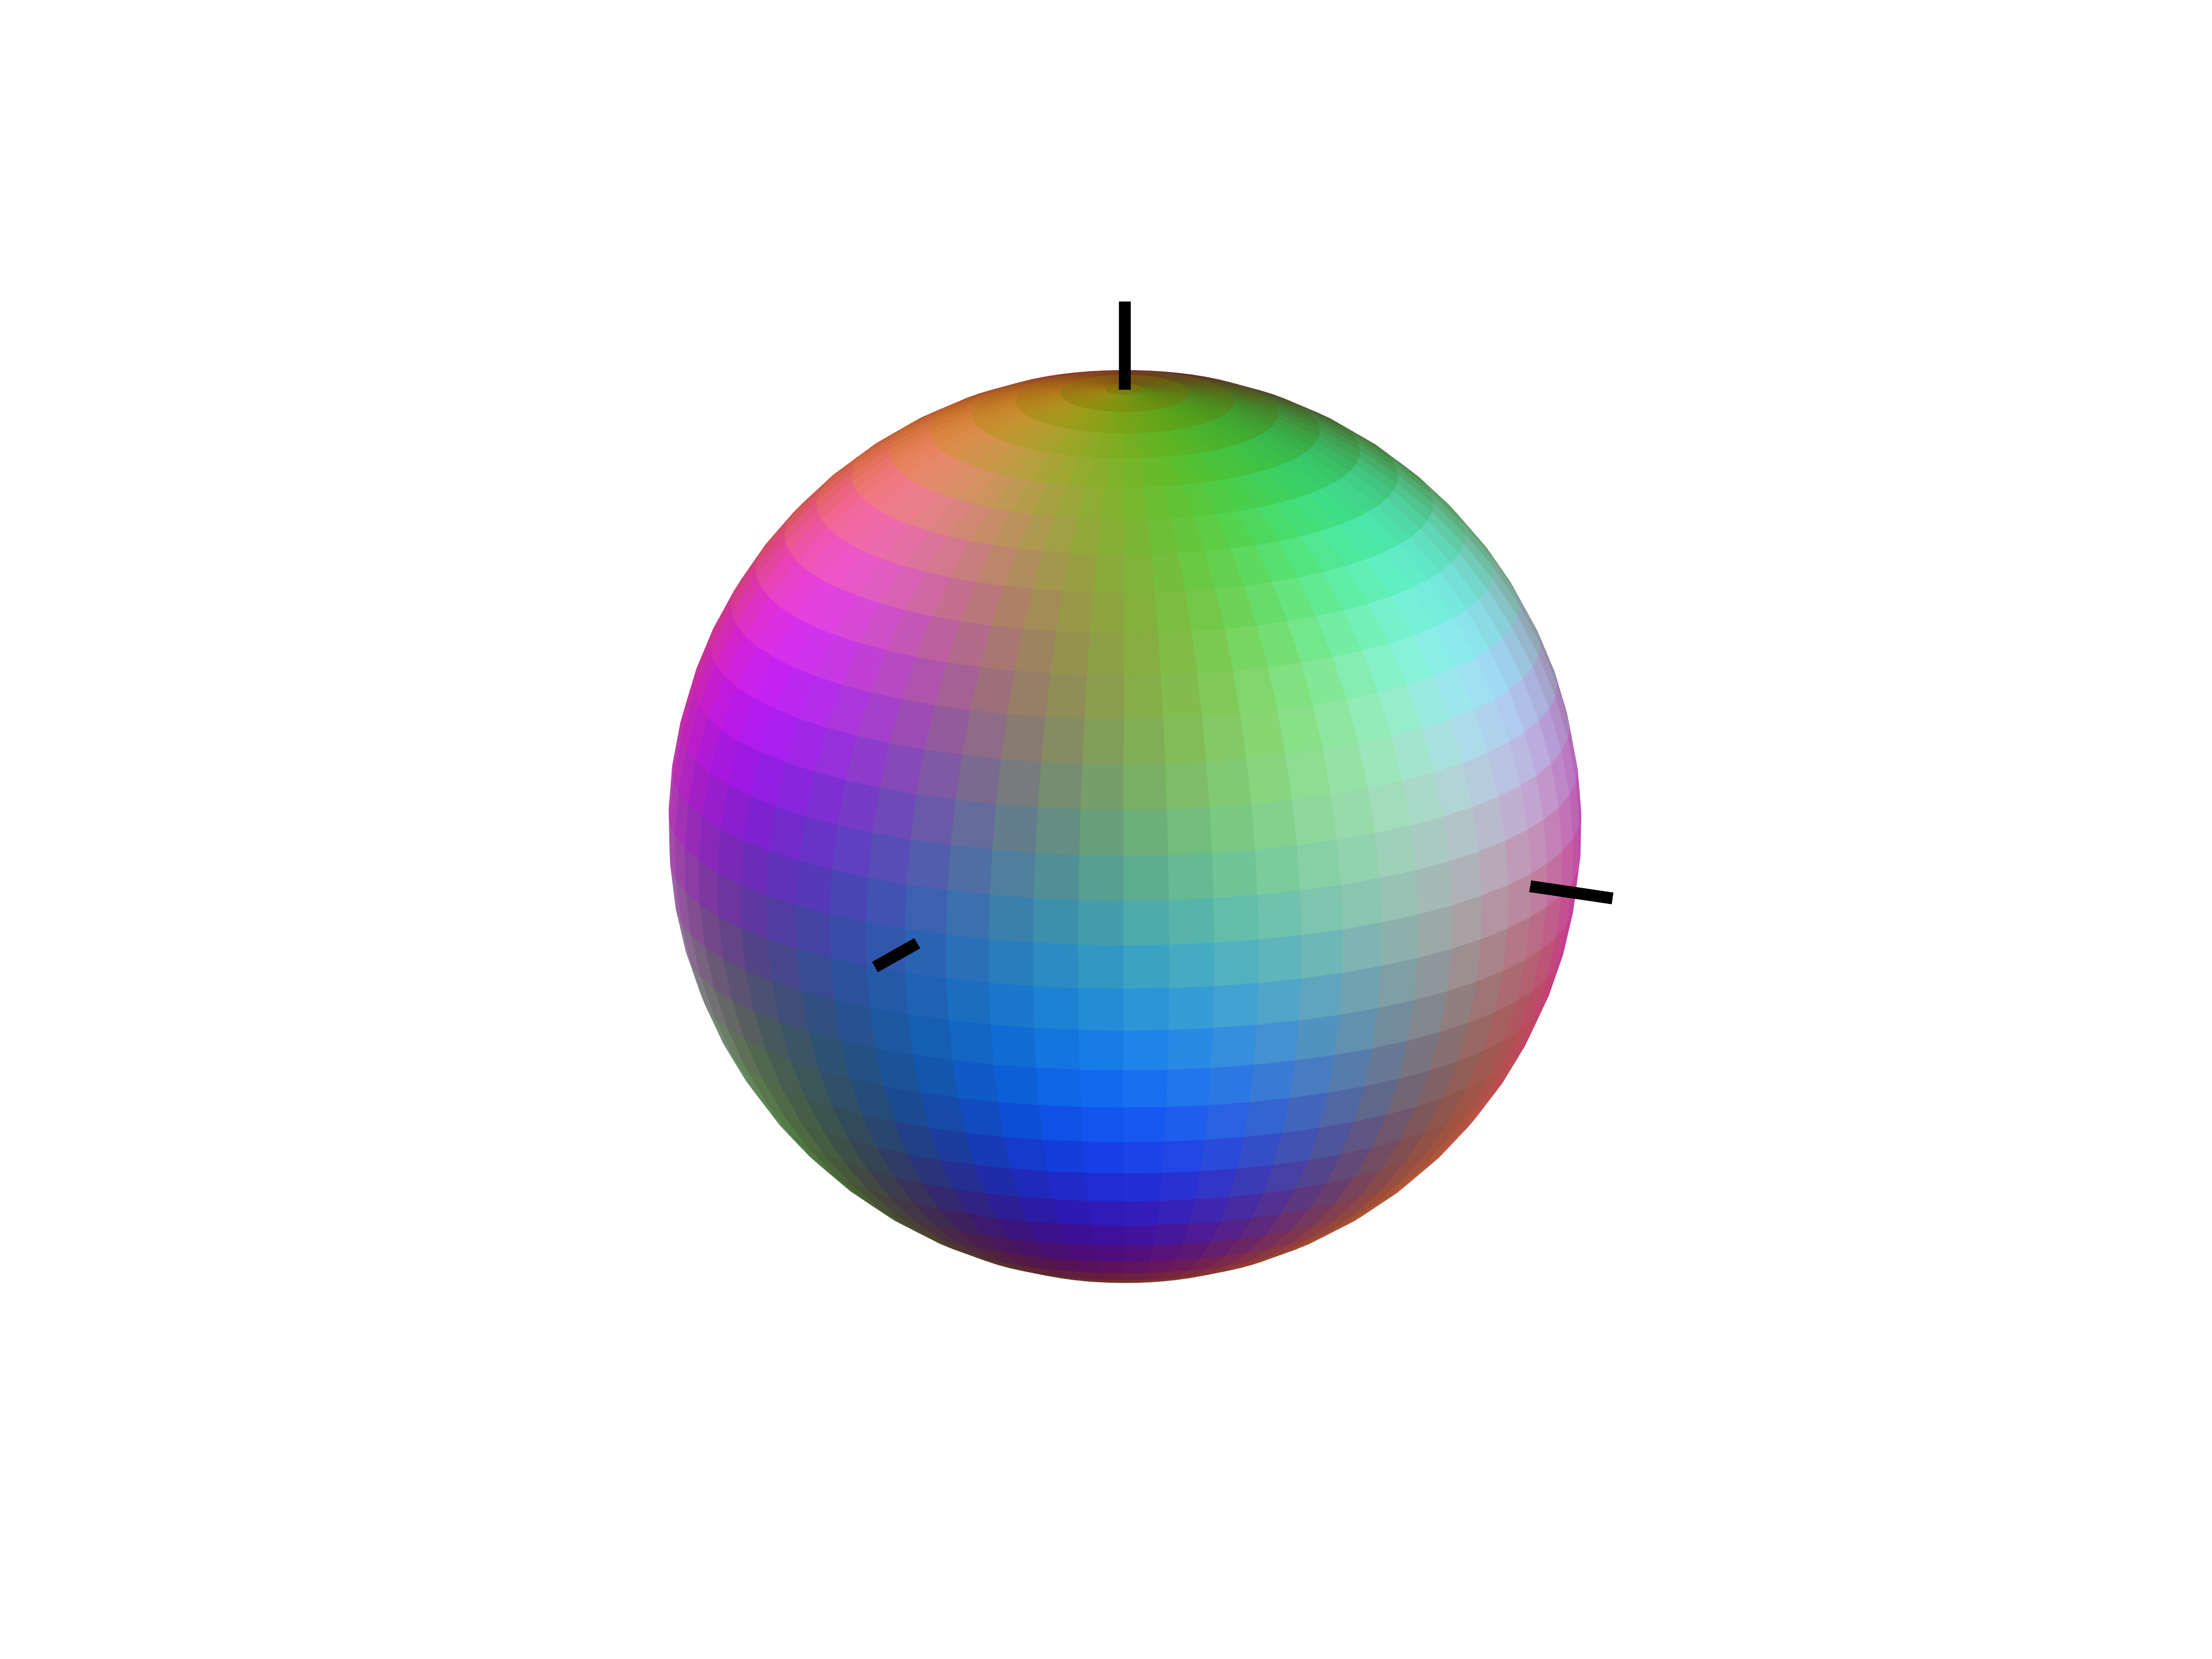
\includegraphics[width=0.33\textwidth]{boys}
		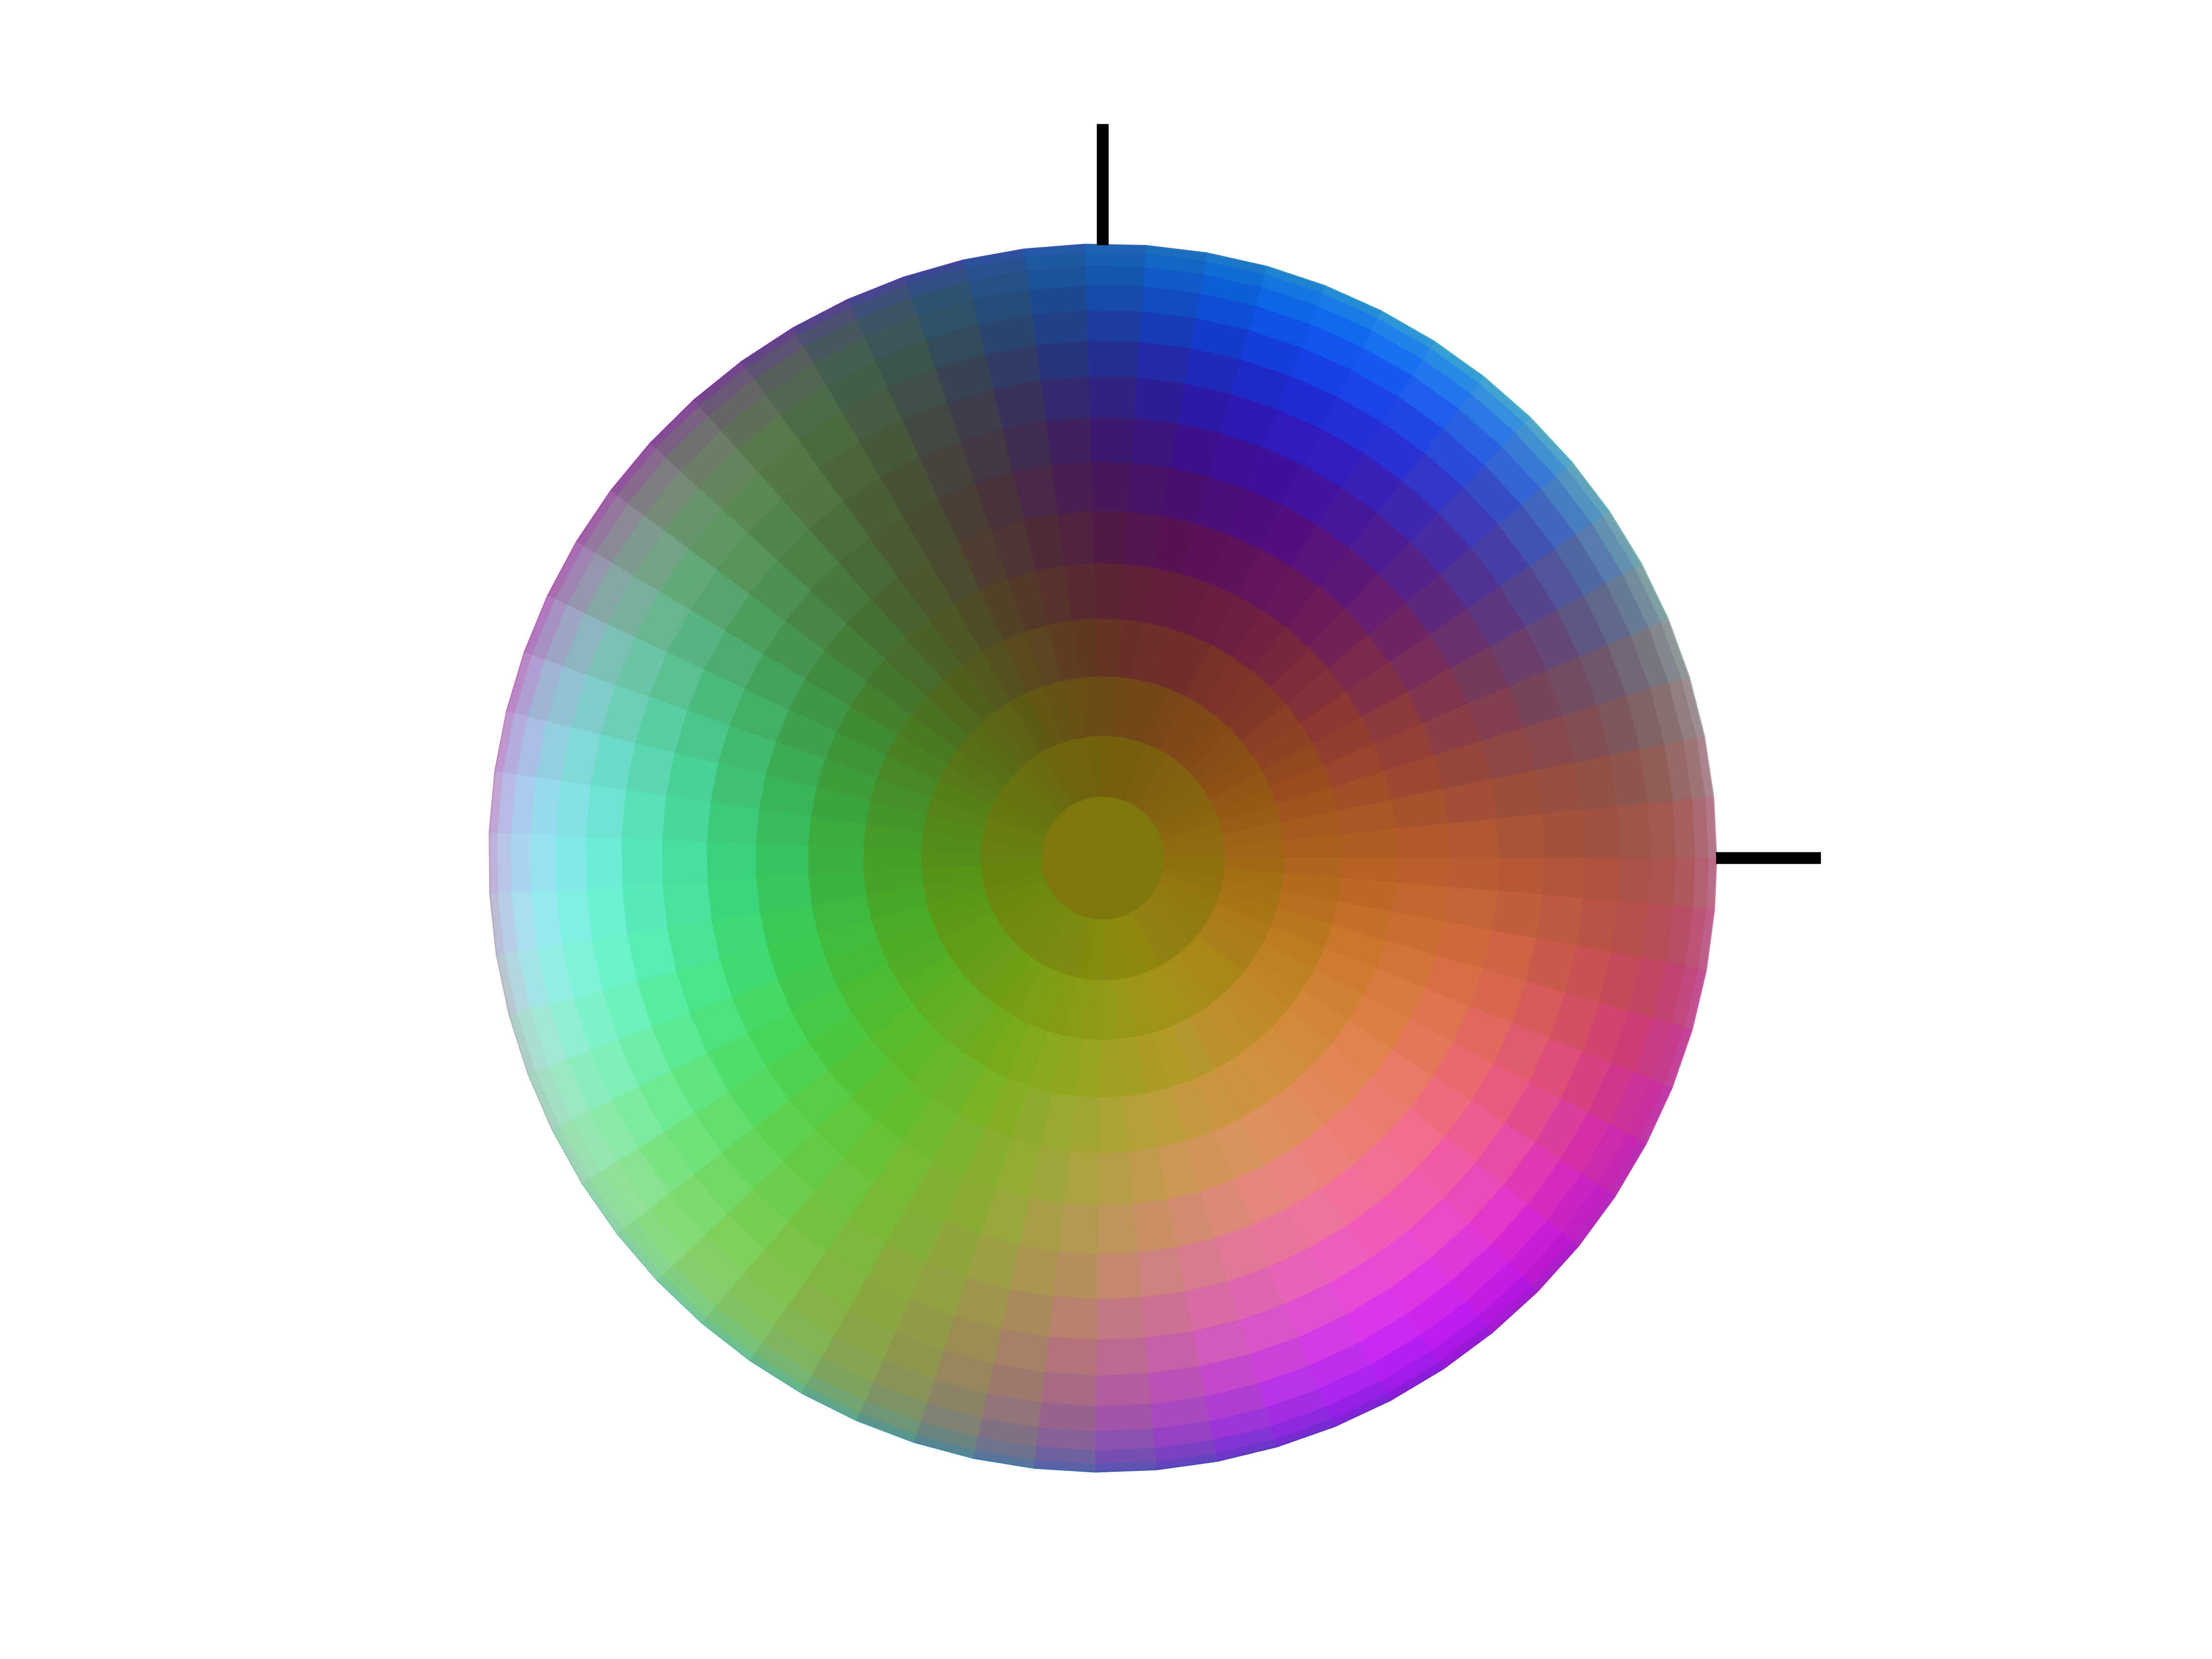
\includegraphics[width=0.3\textwidth]{boys_zIn_yRight}
		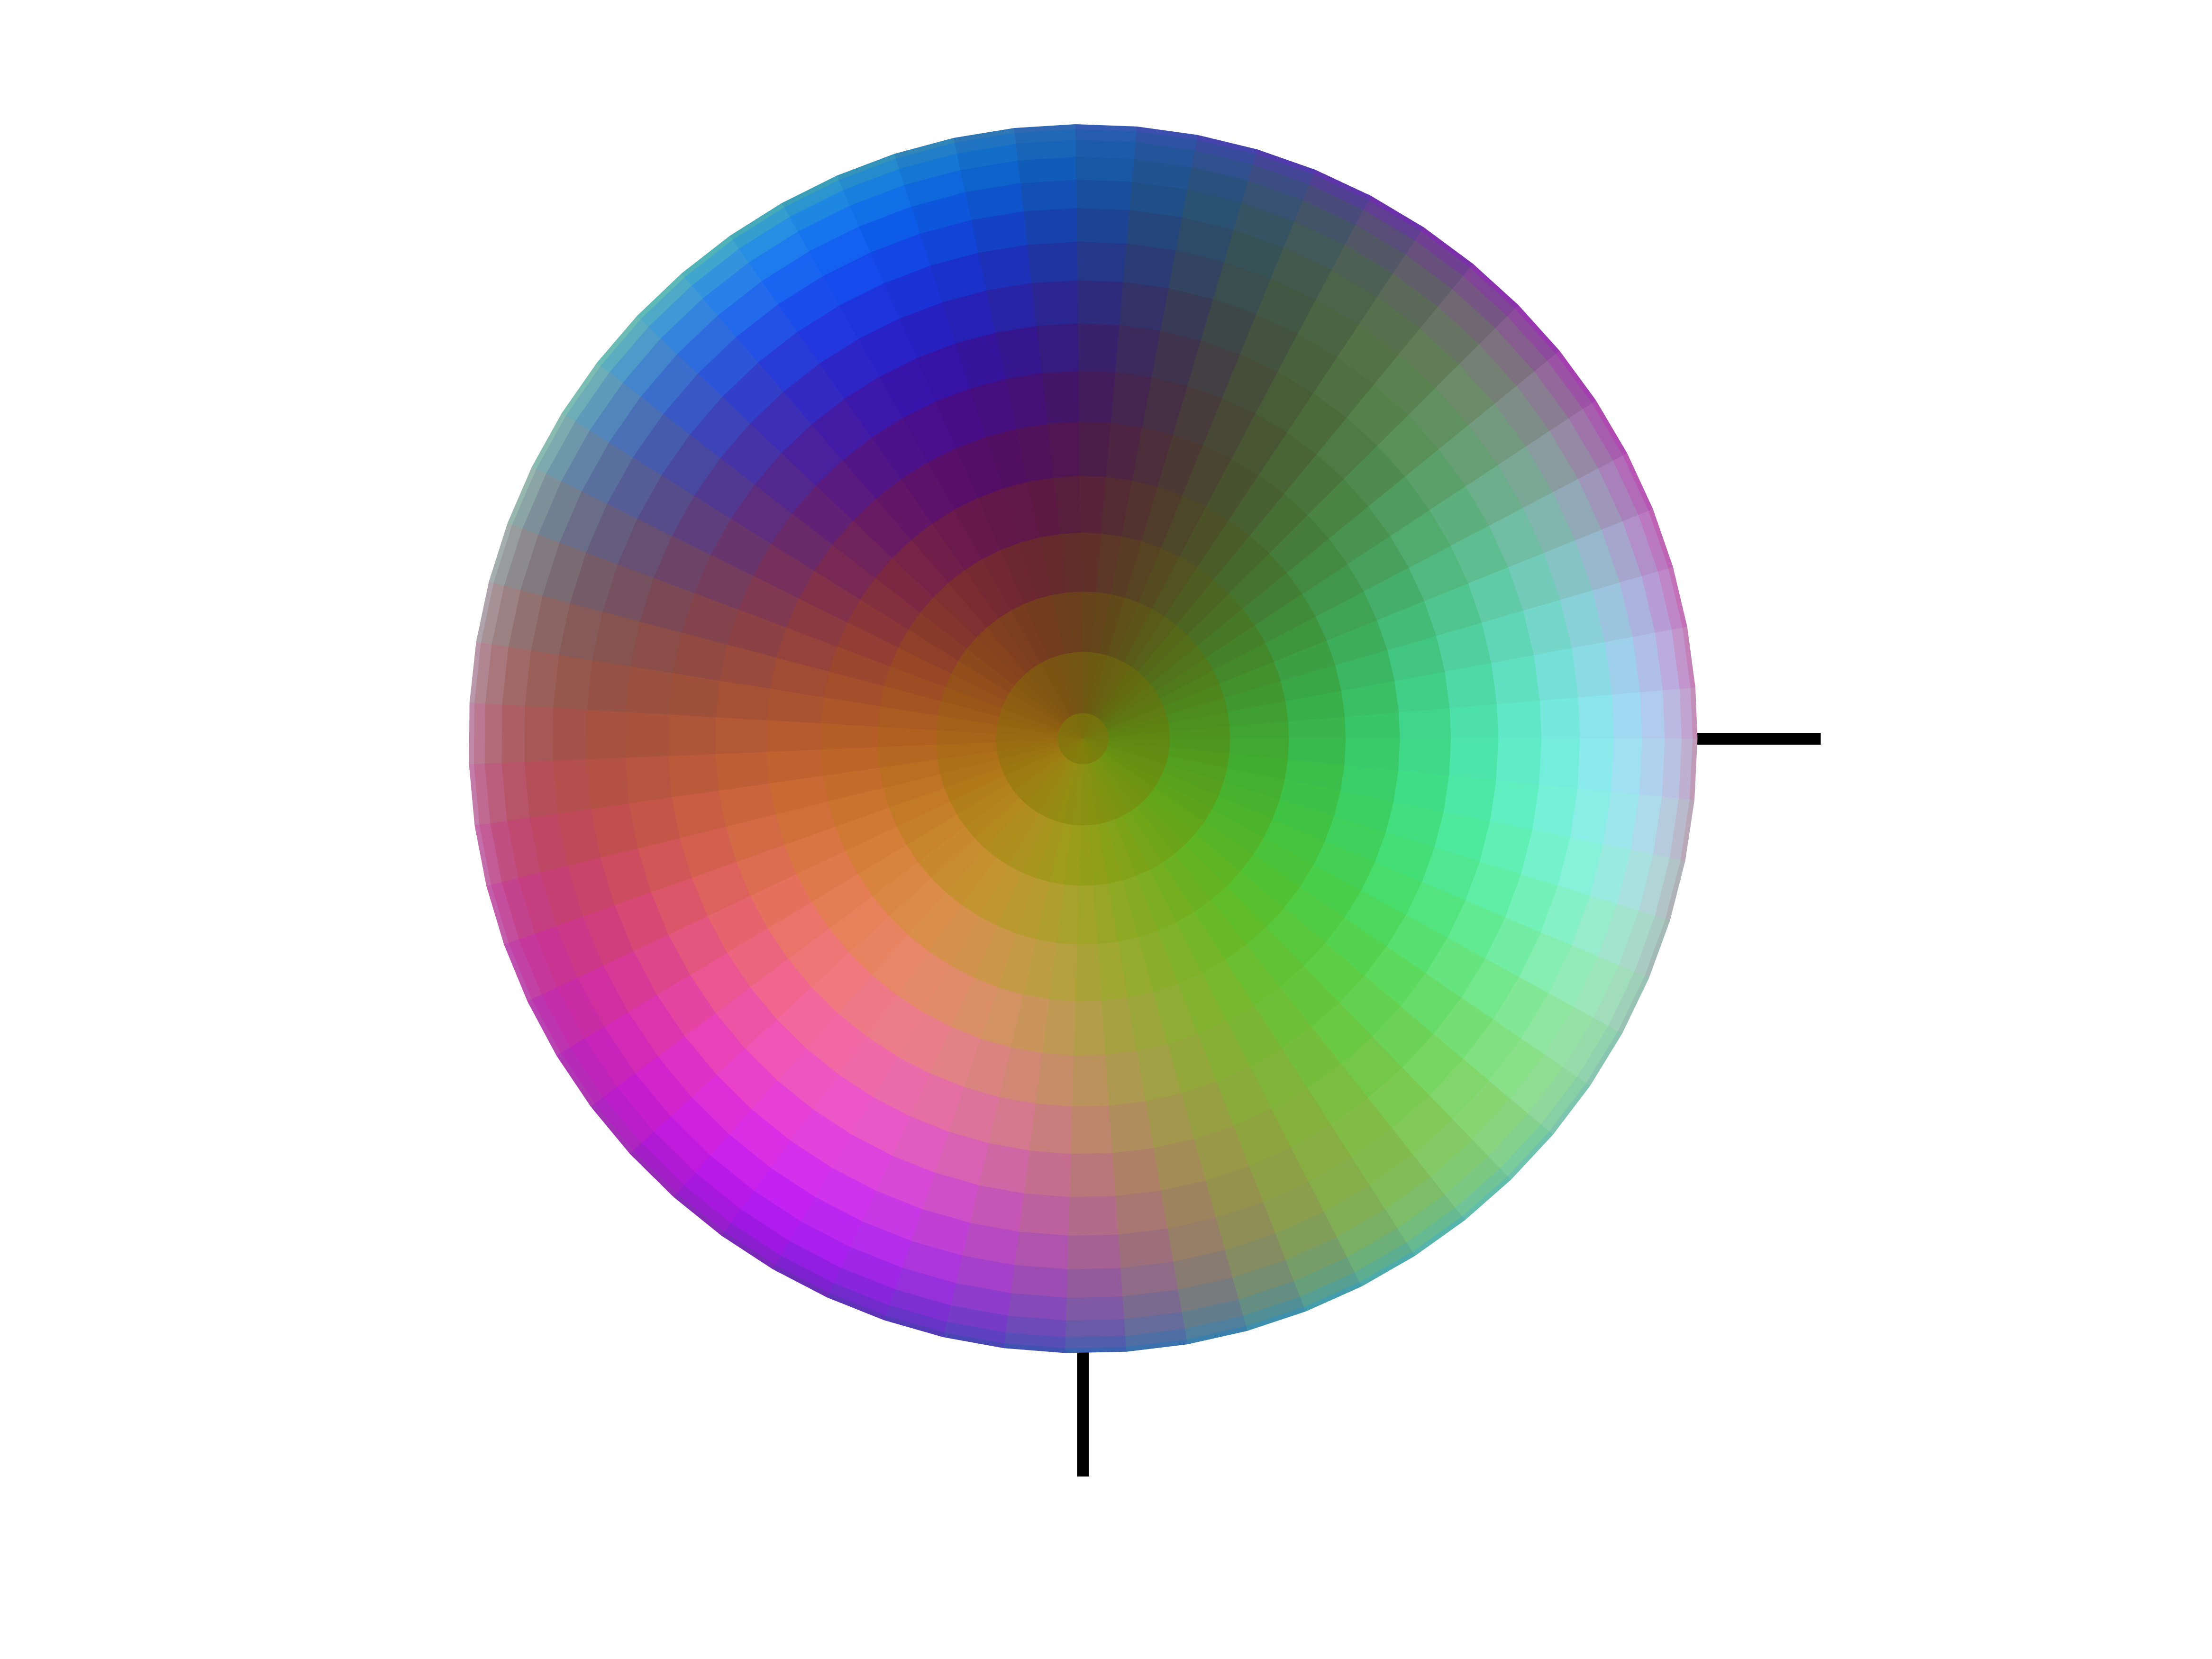
\includegraphics[width=0.3\textwidth]{boys_zOut_yRight}
		\caption{Boy's surface method, colored sphere.}
	\end{figure}

\section{Data acquirement}
We converted Digital Imaging and Communications in Medicine (DICOM) file of brain scans, which is presented in 55-slice into Neuroimaging Informatics Technology Initiative (NIFTI) file. Figure~\ref{fig:2} is the presentation of 55 slices of brain scan.

\begin{figure}[ht]
    \centering
    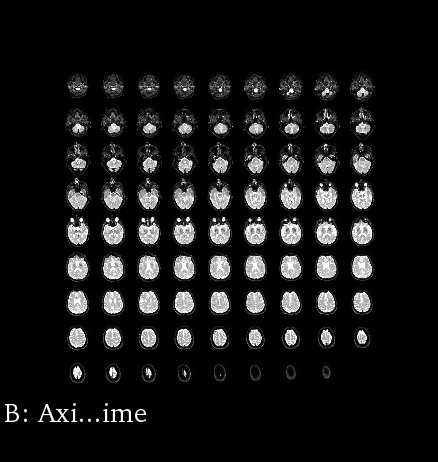
\includegraphics[width = 0.6\columnwidth]{2}
    \caption{ Slice of DICOM  Source:  \cite{???}}
    \label{fig:2}
\end{figure}	

Our first step is brain extraction, using the suitable threshold, which removes non-brain tissue to help with the brain data acquirement. Then we used extracted part to calculate Fractional Anisotropy (FA) and Mean Diffusivity (MD) with the help of FMRIB Software Library (FSL) tool. Finally, we got the Eigenvalues Variance(normalized) and Eigenvalues Mean in the NIFTI files. As Figure~\ref{fig:3} shown, A is the fractional anisotropy value mapping on the green scale; B is the mean diffusivity value mapping on the red scale.
\begin{figure}[ht]
    \centering
    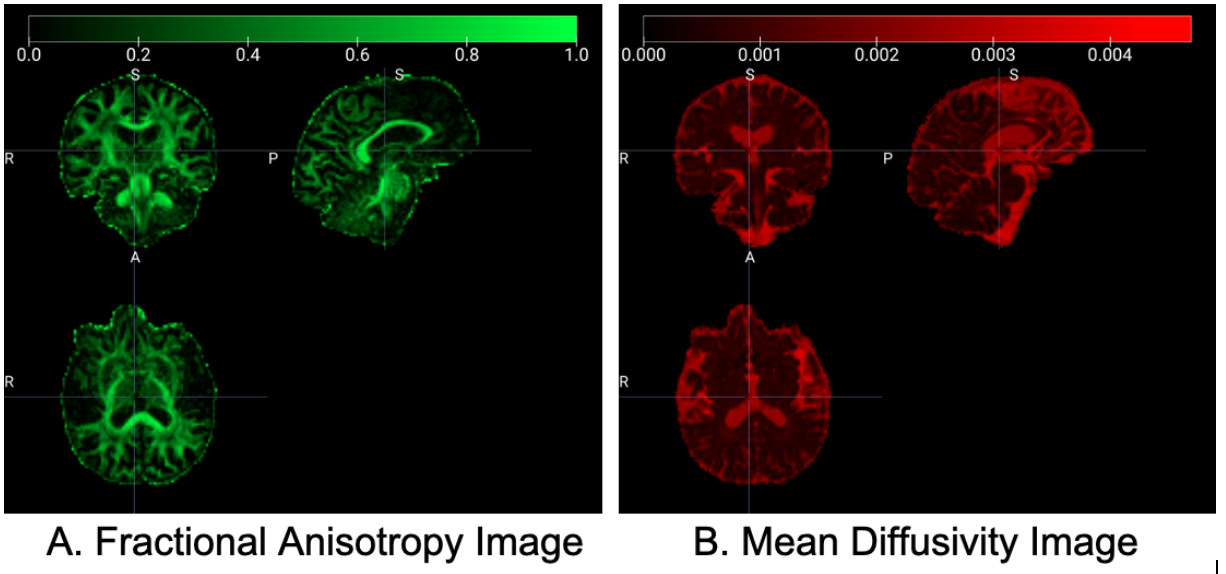
\includegraphics[width = 0.7\columnwidth]{3}
    \caption{ Fractional Anisotropy image and Mean Diffusivity image.}
    \label{fig:3}
\end{figure}	

\section{Rendering}

The brain map read by CGV framework is a TrackVis (trk) file. The data of position is stored in TrackVis file one by one according to the order of the tracts.  Each tract stores two kinds of information, including the offset and the number of points on the current tract, as “Tract (offset, size)”. The Figure~\ref{fig:4} shows the storage mode of TrackVis file. The data read from the NIFTI file with a pointer is in the order of the directory. The storage mode is based on Random Access Storage, i.e., the first dimension to be filled is “x-dimension”, from left to right, then “y-dimension” from posterior to anterior, then “z-dimension”, from inferior to superior. We got the brain data as (116, 116, 80, 55). The first three dimensions are the size of the full volume data in the xyz direction, and the fourth dimension is assumed to refer to time, which also represents the number of slices. The calculated FA and MD data are both with (116, 116, 80, 1). The stored data type is float. The number of voxels is 1,076,480.

\begin{figure}[ht]
    \centering
    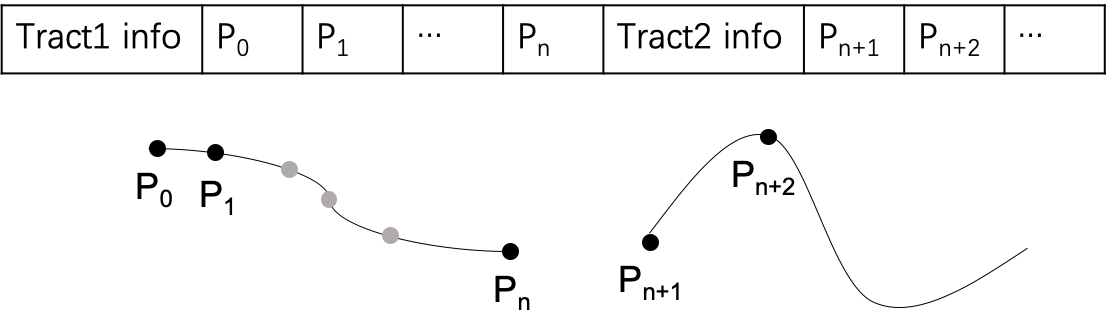
\includegraphics[width = 0.8\columnwidth]{4}
    \caption{Storage mode of TrackVis file.}
    \label{fig:4}
\end{figure}	

In order to access a one-to-one correspondence between the FA/MD data and the brain tract positions, we calculated the bounding box of FA/MD data, which is to eliminate the voxels whose FA and MD values are 0. After that we ordered the eliminated data again and stored them in a new vector. The dimension of the processed data is (70, 82, 76, 1) on xyzt dimension. The number of voxels is 436,240. (Figure~\ref{fig:5})

\begin{figure}[ht]
    \centering
    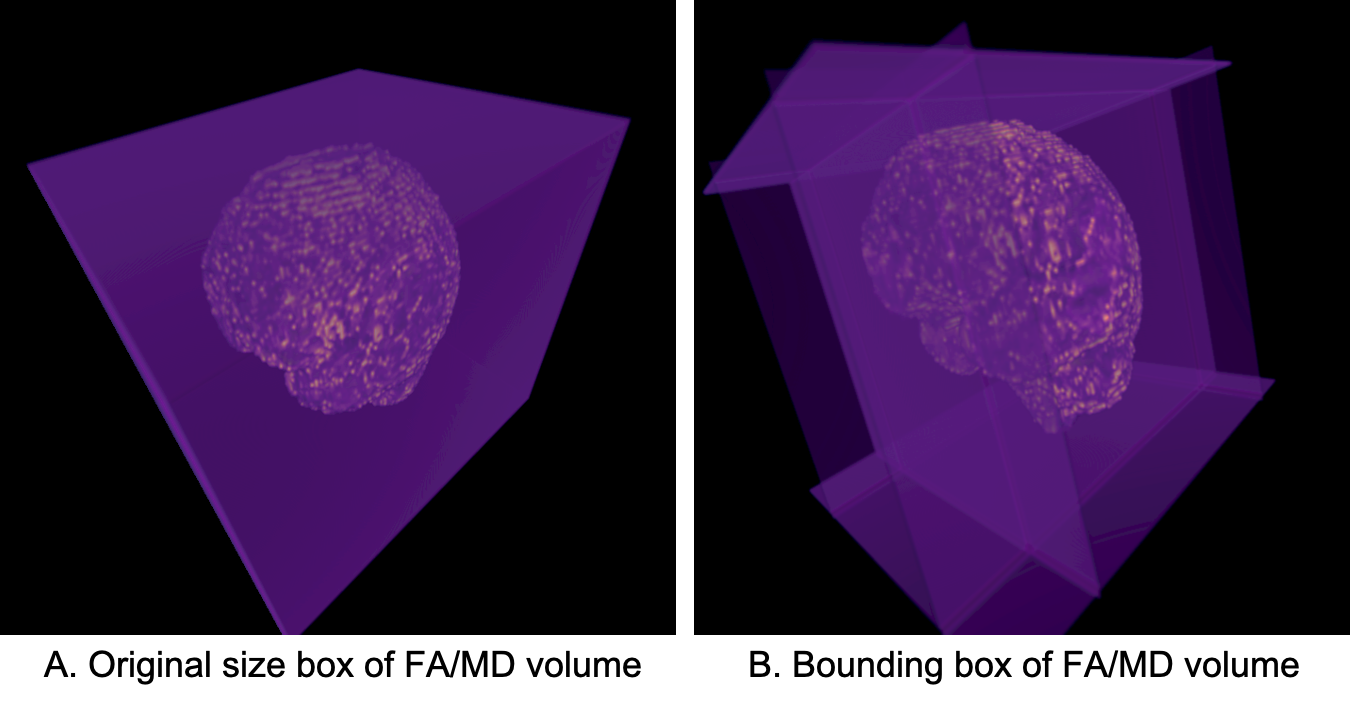
\includegraphics[width = 0.8\columnwidth]{5}
    \caption{Sketch of size cutting.}
    \label{fig:5}
\end{figure}	


Since the dimensional order of data rendering in Opengl is in xzy-oder, and the storage order of FA/MD data are in xyz-order, we have transformed the data through the corresponding between coordinate and index. As it shown in Figure~\ref{fig:6}, we mapped the FA/MD value on tractography volume with size matching and dimension swapping.

\begin{figure}[ht]
    \centering
    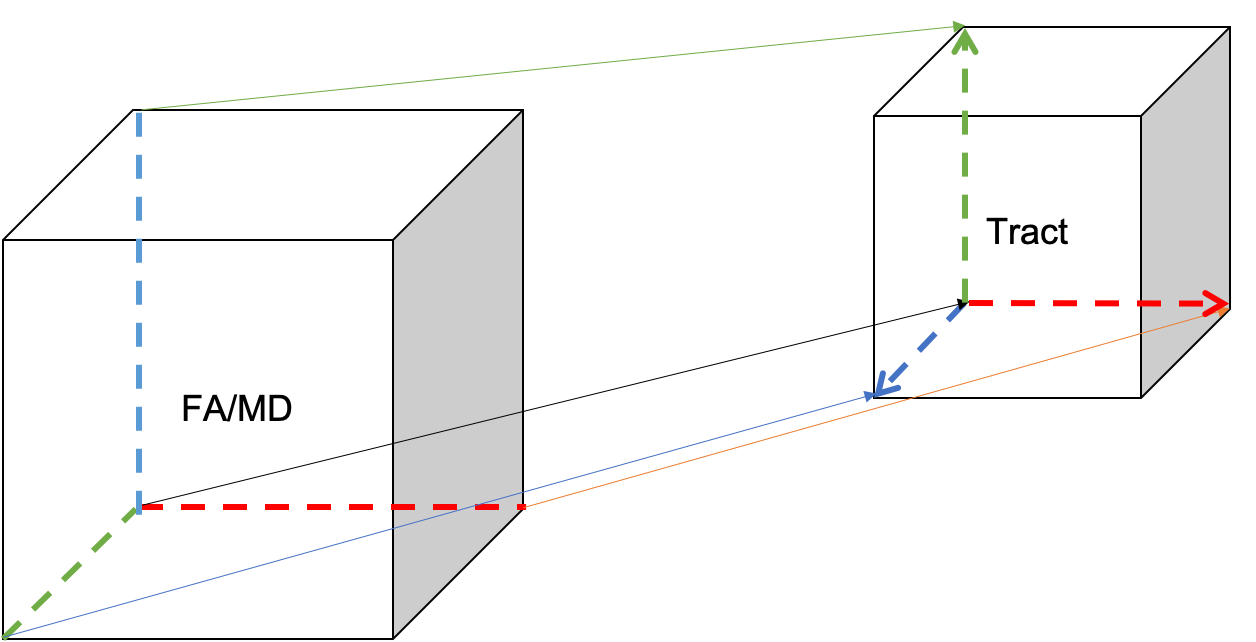
\includegraphics[width = 0.8\columnwidth]{6}
    \caption{Sketch of size matching and dimension swapping between FA/MD and Tractography.}
    \label{fig:6}
\end{figure}	

After mapping FA and MD to different color map values and mapping them to the corresponding tract positions, we get ten different brain maps. As it shown in the Figure~\ref{fig:7} and \ref{fig:8}.

\begin{figure}[ht]
    \centering
    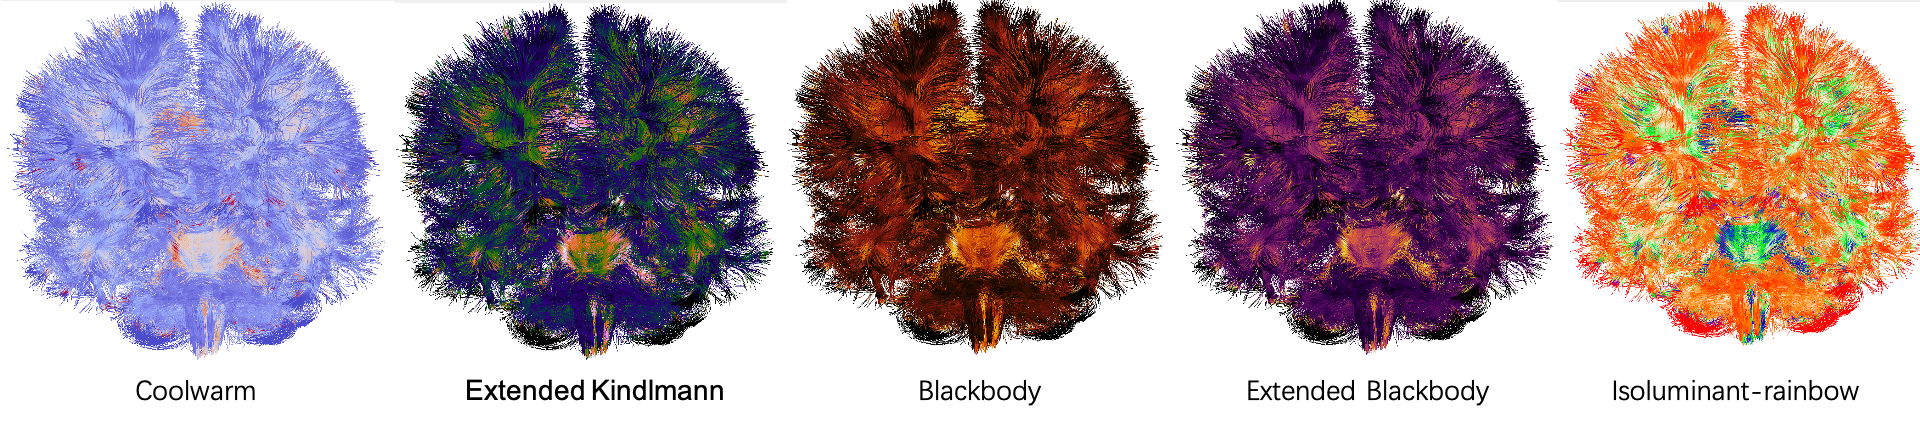
\includegraphics[width = 0.9\columnwidth]{7}
    \caption{Tractography of FA in different colormap.}
    \label{fig:7}
\end{figure}

\begin{figure}[ht]
    \centering
    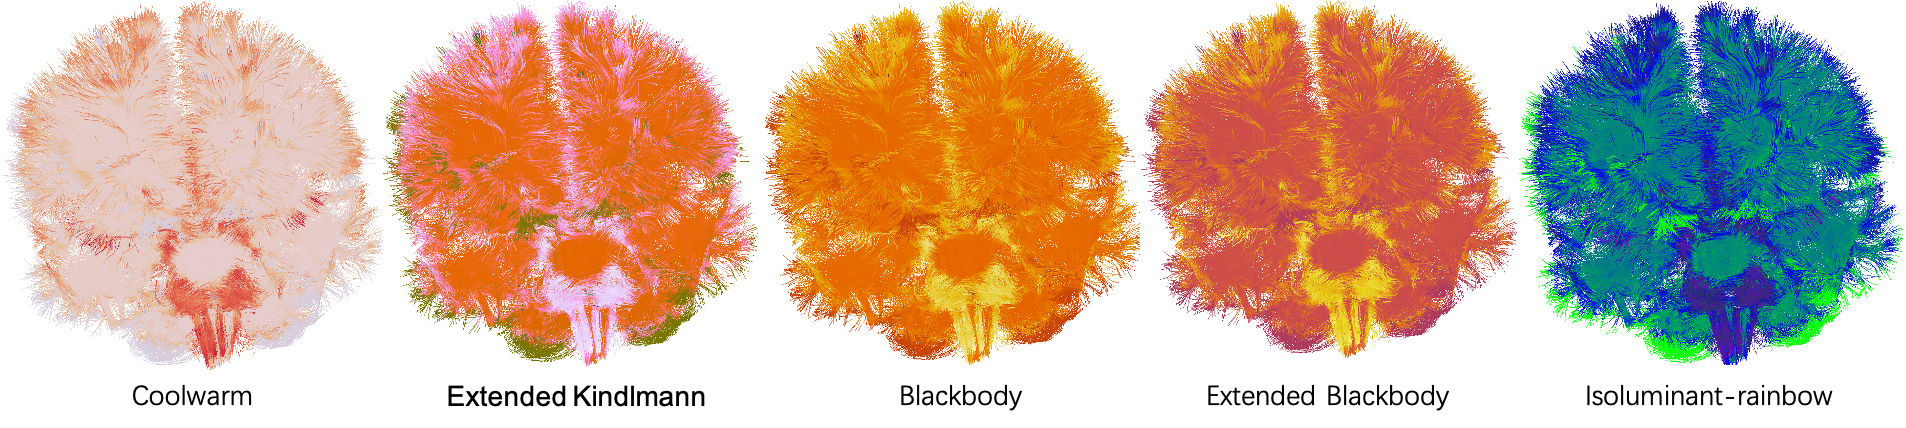
\includegraphics[width = 0.9\columnwidth]{8}
    \caption{Tractography of MD in different colormap.}
    \label{fig:8}
\end{figure}

\chapter{Evaluation}

The first objective of this chapter is to discuss what users would want to achieve when using the tractography images. Users of such visualizations range from medical doctors and researchers to biologists and neuroscientists. In addition to different viewpoints, users from different categories have different capabilities and resources. For instance, it can be expected that medical doctors have more critical time constraints than researchers. As another example, it is likely that neuroscientists are more acquainted with computer tools, data processing and complex user interfaces.

The second objective is to discuss how we can compare the effect of color mapping as well as the choice of attribute (FA or MD) on user's success in retrieving information. To this end, we design a user study through a questionnaire. The questionnaire should provide statistical information about how each combination of the alternatives affect user's success. 

\section{Task Characteristics}

The term ``task" refers to a specific objective of a user. Chen et al. \cite{chen} identified four major task types : 
\begin{enumerate}
	\item Ensemble identification, 
	\item Ensemble comparison, 
	\item Ensemble localization and
	\item Ensemble association.
\end{enumerate}
See Figure~\ref{fig:task-types} for an illustration of the tasks as implemented in \cite{chen}. Following \cite{chen}, we study the first \emph{identification} task type as it is most common in DMRI visualization challenges. 

\begin{figure}[ht]
    \centering
    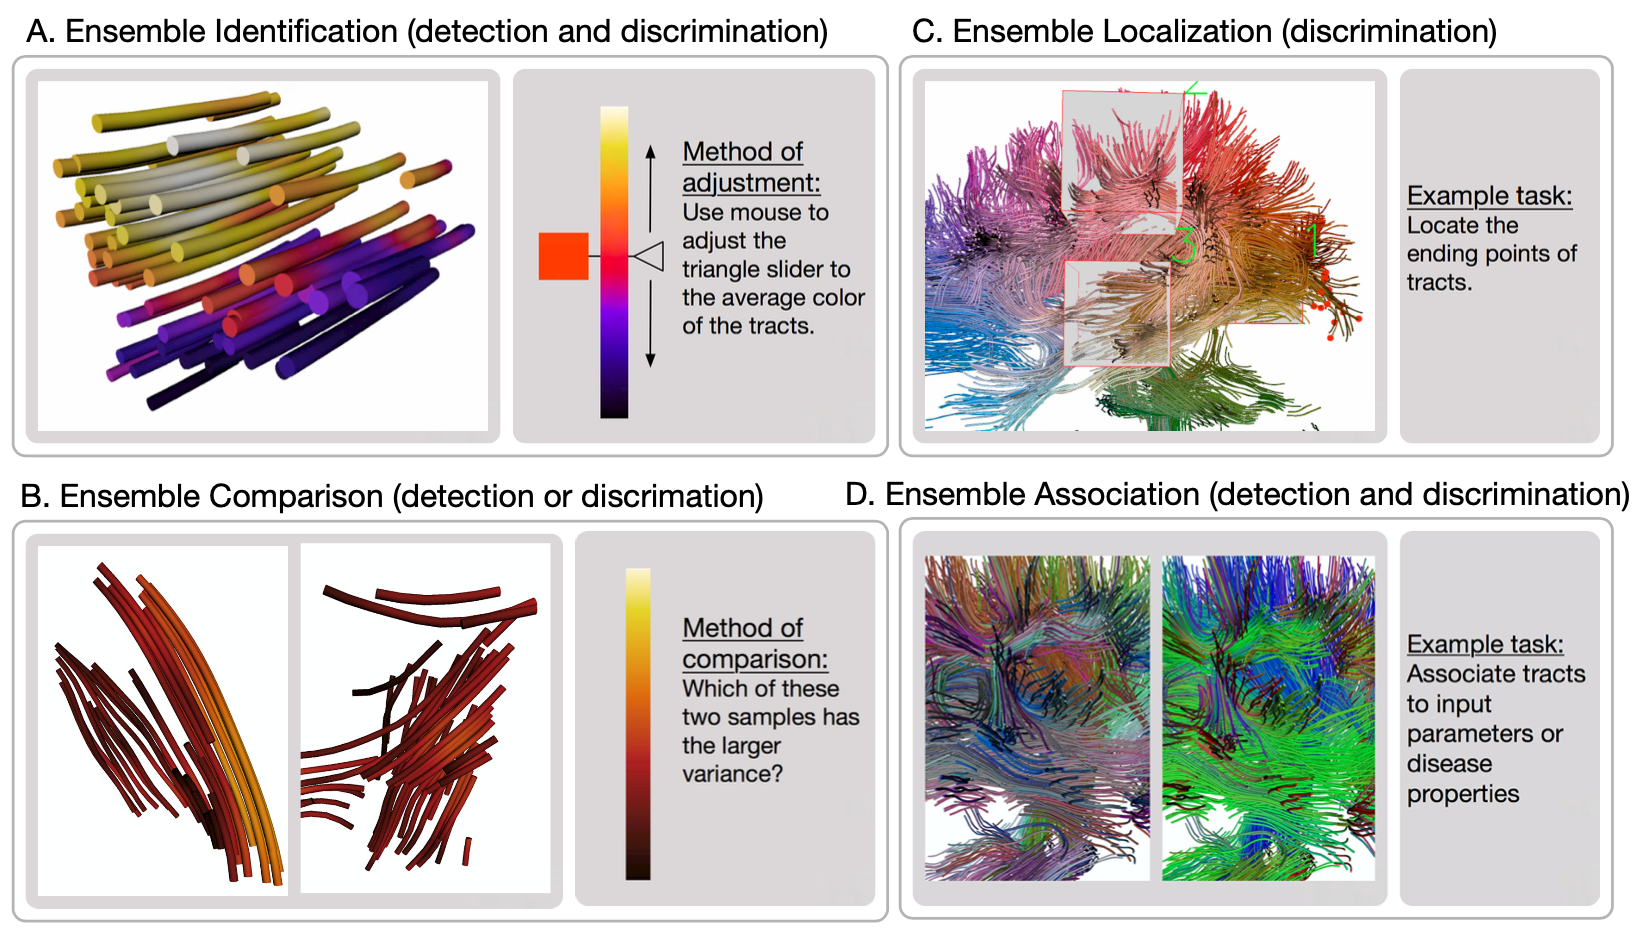
\includegraphics[width = 0.9\columnwidth]{task-types}
    \caption{Illustration of the four task types by example tasks. Source:  \cite{chen}}
    \label{fig:task-types}
\end{figure}

As a starting point for design of the user study, i.e. the questionnaire, the following expectations are considered which are intuitively reasonable and can be verified by a user study.
\begin{enumerate}
	\item A spherical color mapping with higher spatial resolution should help with identification of the orientation of the tracts. Among the colormaps implemented in this work, Boy's surface has higher spatial resolution and is expected to help the user follow the tracts better.
	\item Scalar color mapping based on FA and MD should affect the user's ability to estimate the average over a region.
\end{enumerate}

\section{Task presentation}
He we formulate the specific tasks according to the expectations mentioned in the previous section. The following tasks are inspired by the works of Chen et al. \cite{chen}, Henan et al. \cite{henan} and Borgo et al. \cite{borgo}.

By ``Base Question" we refer to a basic question from which several questions are implemented in the questionnaire.

\paragraph{A. Ensemble Average}

As discussed in Section~\comment{??}, FA and MA are the actual quantities that can be related the state of a region in brain. Clearly, the quantity in a voxel or very small part of the brain does not reveal much. The user likely intends to compare larger regions by estimating a gross or average value of the quantity.
\begin{itemize}
	\item{Task 1:} The base question is: ``What is the average FA/MD values of the tracts?"
	In this task, the participants will be asked to estimate the average FA and MD. The user does the estimation by an image of a small region in brain. Then he/she indicates the answer by choose from a finite number of labels on the colorbar. The instances of this question should include scalar color mappings and the choice of MD or FA (Figure~\ref{fig:task1-fa} and \ref{fig:task1-md}). Each combination should be repeated for several regions to increase reliability. 
     	
\begin{figure}[ht]
    \centering
    \begin{subfigure}[b]{0.45\textwidth}
    	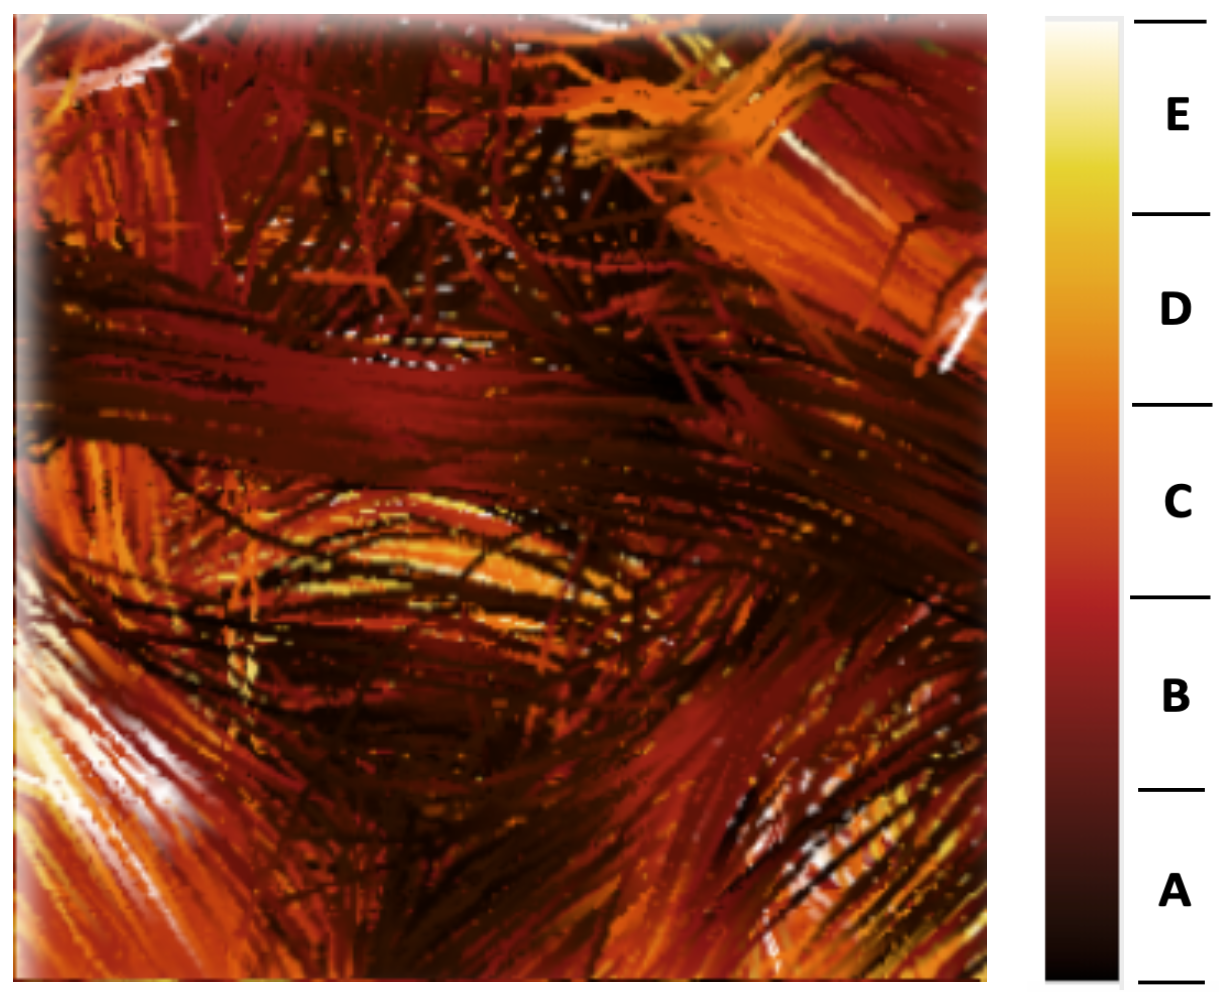
\includegraphics[width =  \columnwidth]{blackbody-fa}
	\caption{ }
    \end{subfigure}
    \hspace{0.3cm}
    \begin{subfigure}[b]{0.45\textwidth}
    	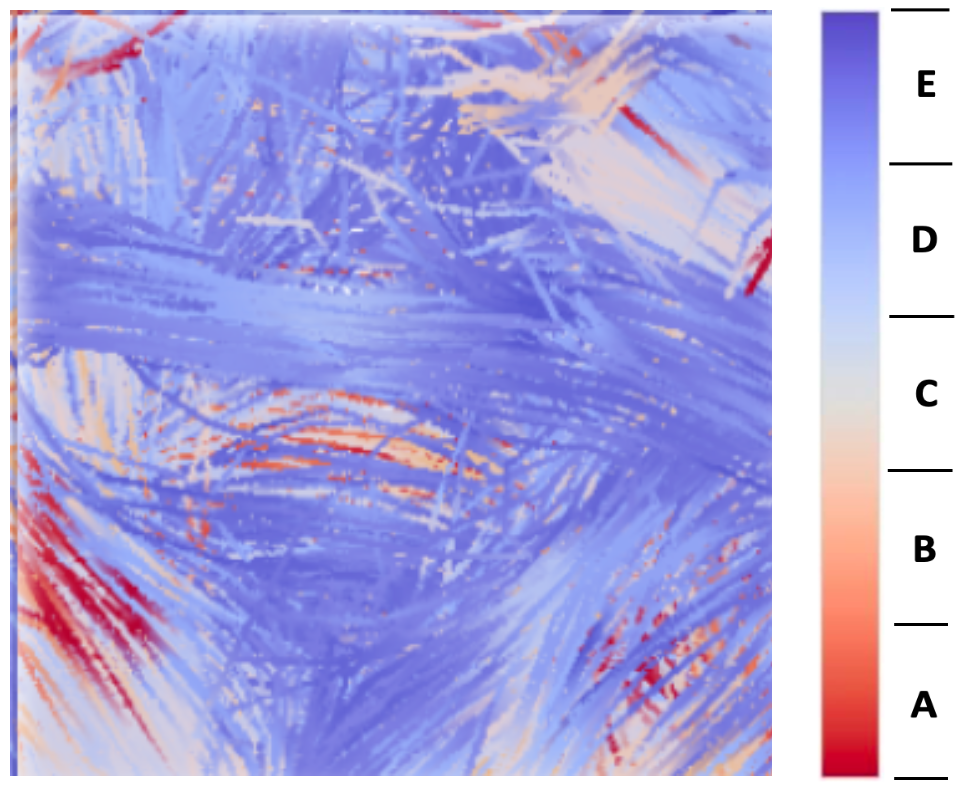
\includegraphics[width =  \columnwidth]{coolwarm-fa}
	\caption{ }
    \end{subfigure}	
    \begin{subfigure}[b]{0.45\textwidth}
    	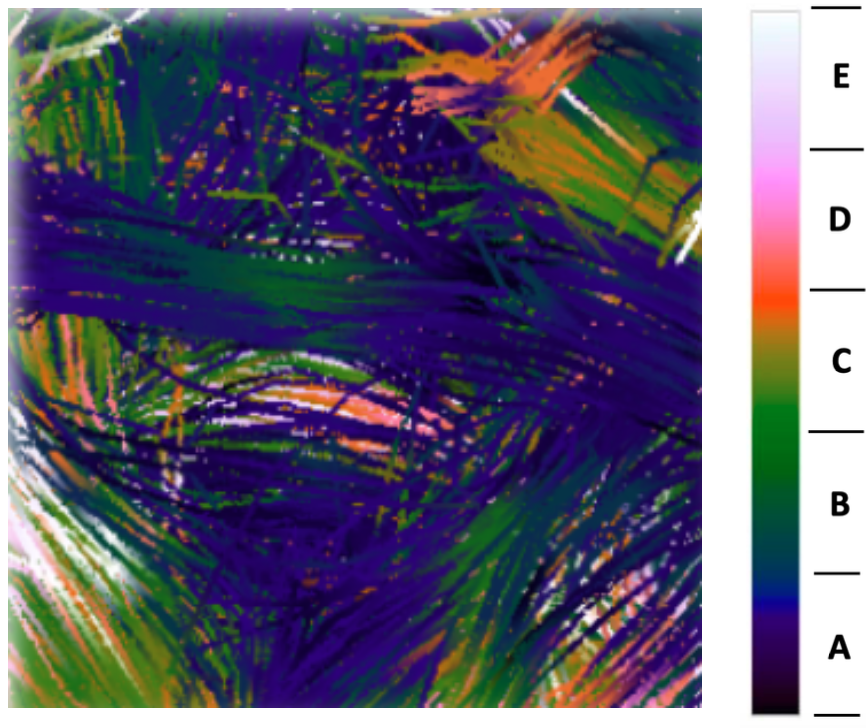
\includegraphics[width =  \columnwidth]{ekindlmann-fa}
	\caption{ }
    \end{subfigure}	
    \hspace{0.3cm}	
    \begin{subfigure}[b]{0.45\textwidth}
    	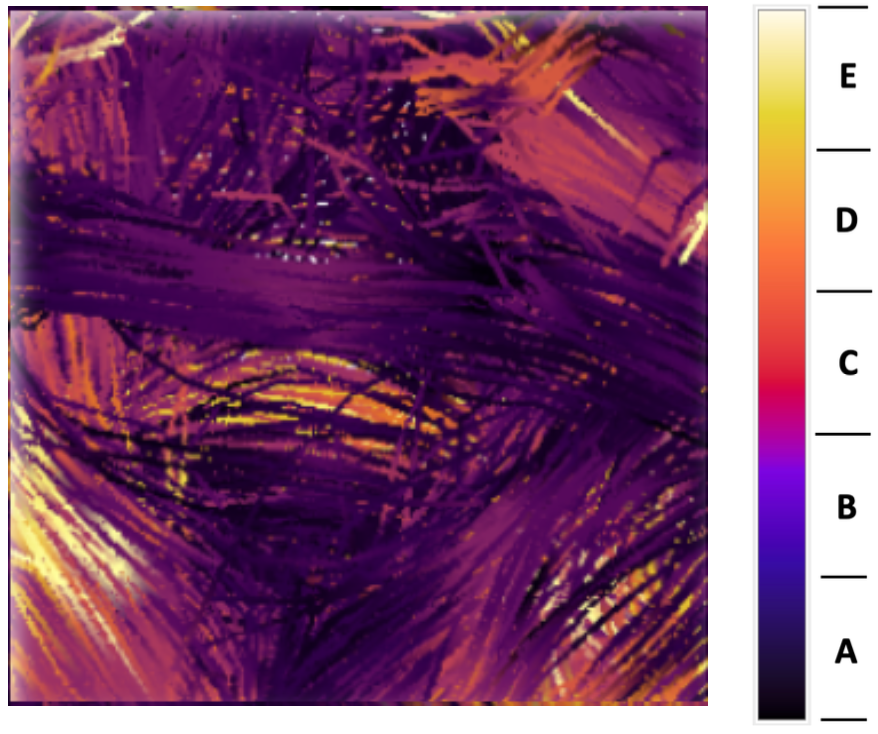
\includegraphics[width =  \columnwidth]{eblackbody-fa}
	\caption{ }
    \end{subfigure}
    \begin{subfigure}[b]{0.45\textwidth}
    	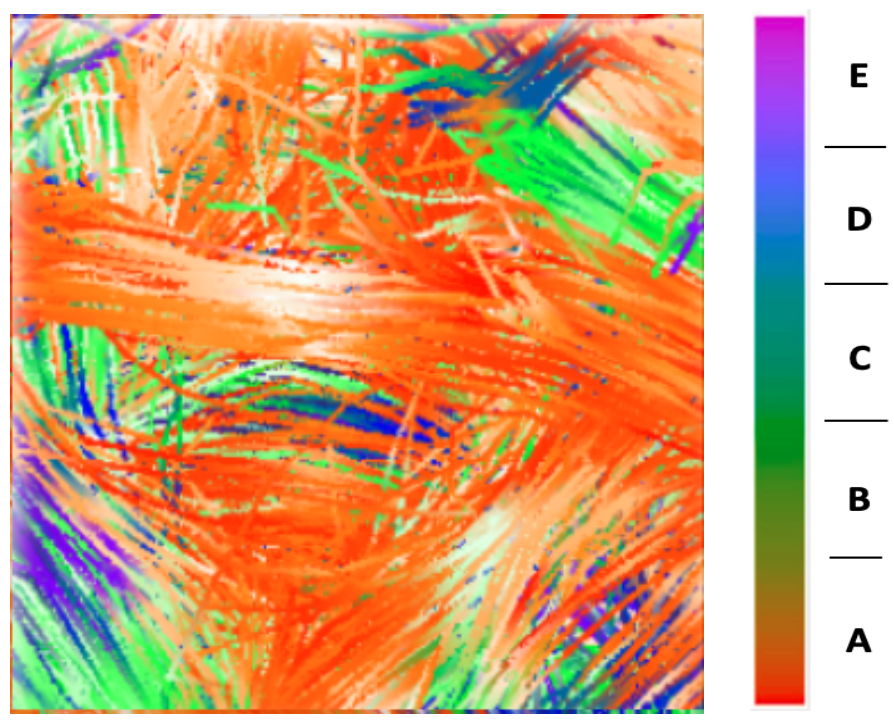
\includegraphics[width =  \columnwidth]{isorainbow-fa}
	\caption{ }
    \end{subfigure}	
    \caption{Illustration of the questions for back of the brain, based on Task 1 for average FA and a)Blackbody b)Coolwarm c)Extended Kindlmann d)Extended Blackbody e)Isoluminant-rainbow }
    \label{fig:task1-fa}
\end{figure}

\begin{figure}[ht]
    \centering
    \begin{subfigure}[b]{0.45\textwidth}
    	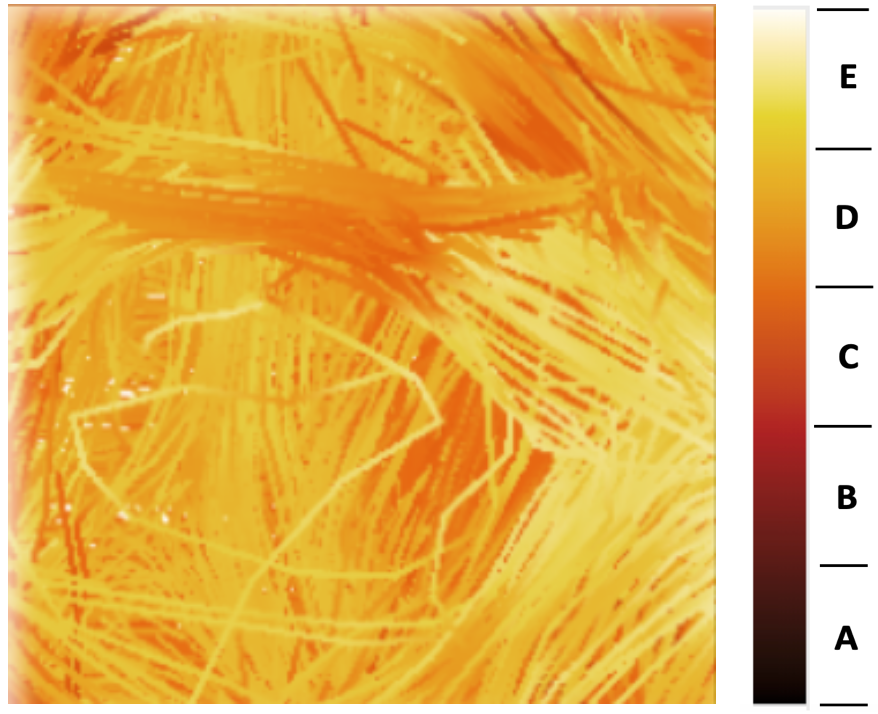
\includegraphics[width =  \columnwidth]{blackbody-md}
	\caption{ }
    \end{subfigure}
    \hspace{0.3cm}
    \begin{subfigure}[b]{0.45\textwidth}
    	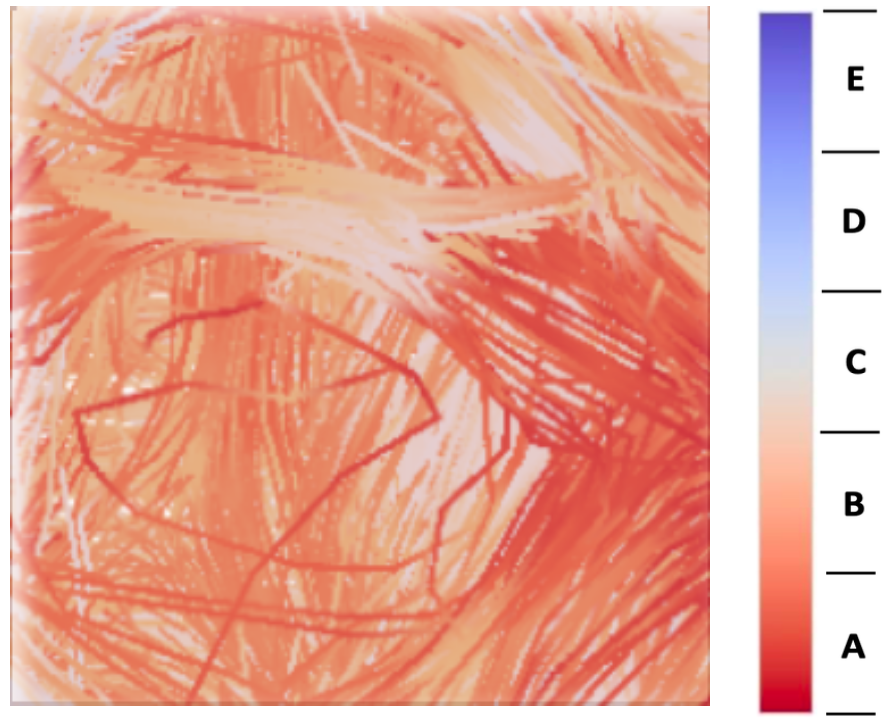
\includegraphics[width =  \columnwidth]{coolwarm-md}
	\caption{ }
    \end{subfigure}	
    \begin{subfigure}[b]{0.45\textwidth}
    	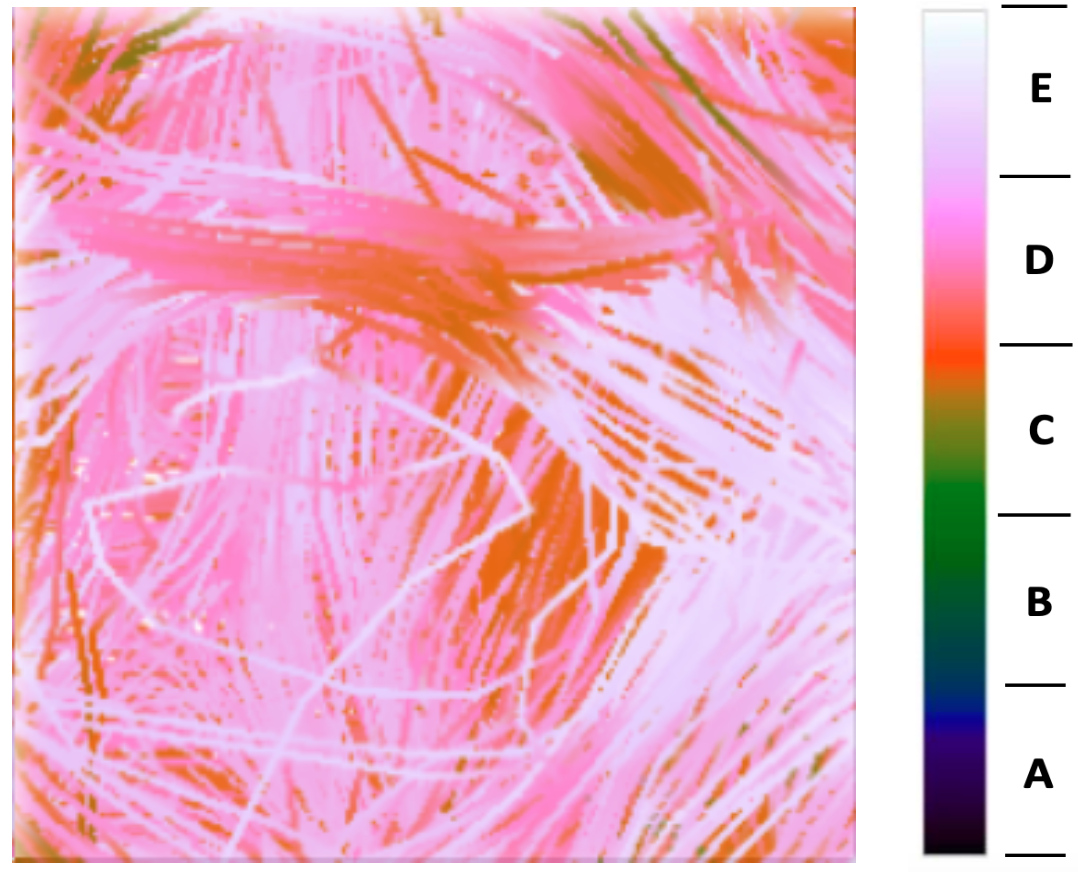
\includegraphics[width =  \columnwidth]{ekindlmann-md}
	\caption{ }
    \end{subfigure}	
    \hspace{0.3cm}	
    \begin{subfigure}[b]{0.45\textwidth}
    	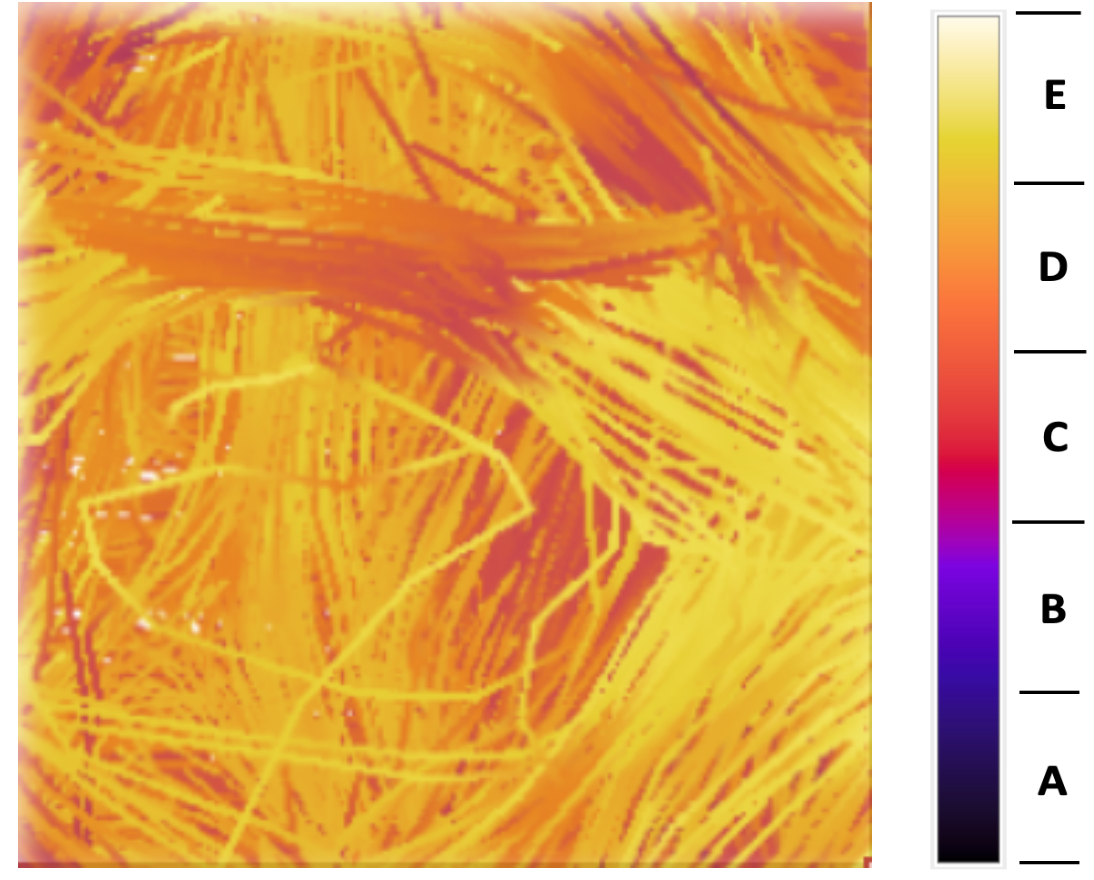
\includegraphics[width =  \columnwidth]{eblackbody-md}
	\caption{ }
    \end{subfigure}
    \begin{subfigure}[b]{0.45\textwidth}
    	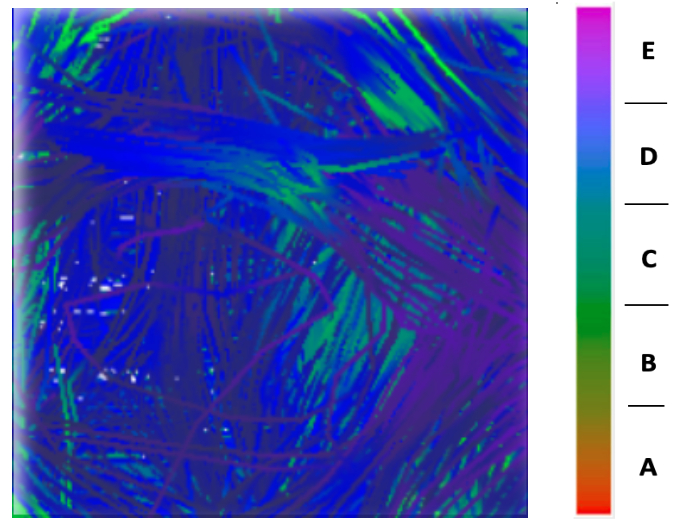
\includegraphics[width =  \columnwidth]{isorainbow-md}
	\caption{ }
    \end{subfigure}	
    \caption{Illustration of the questions for back of the brain, based on Task 1 for average MD and a)Blackbody b)Coolwarm c)Extended Kindlmann d)Extended Blackbody e)Isoluminant-rainbow }
    \label{fig:task1-md}
\end{figure}

	
	\item{Task 2:} The base question is: ``Which average FA/MD is greater?" 
	In this task, the participants were asked to choose the greater average FA/MD between two regions marked on the whole brain image (Figure~\ref{fig:task2}) Similar to Task 1, a number of questions are generated from this base question. 

\begin{figure}[t]
	\centering
	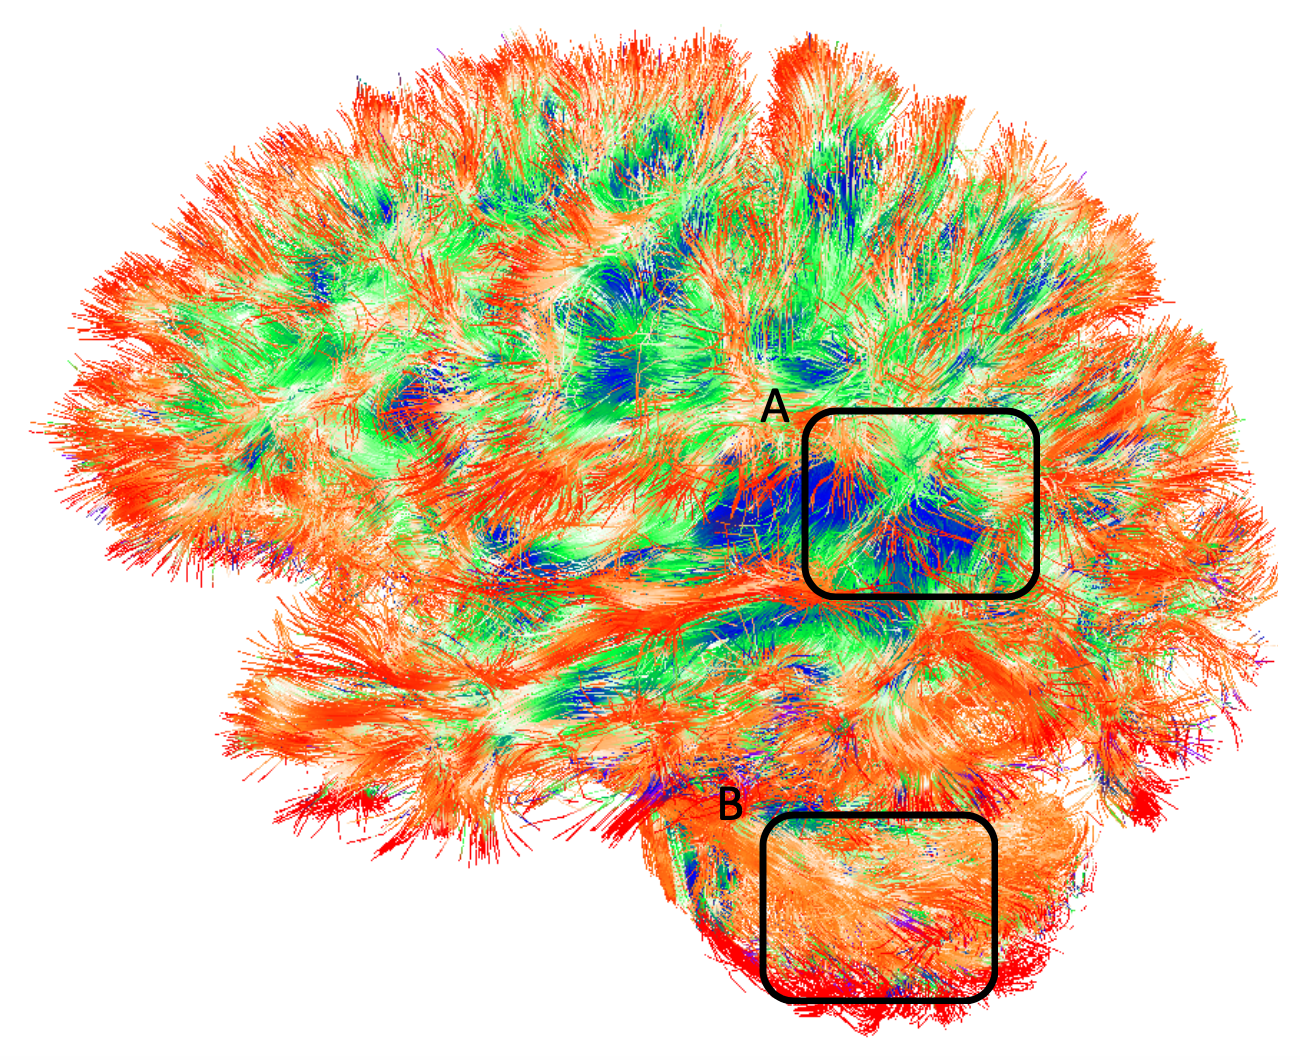
\includegraphics[width=0.8\columnwidth]{isorainbow-fa-task2}
	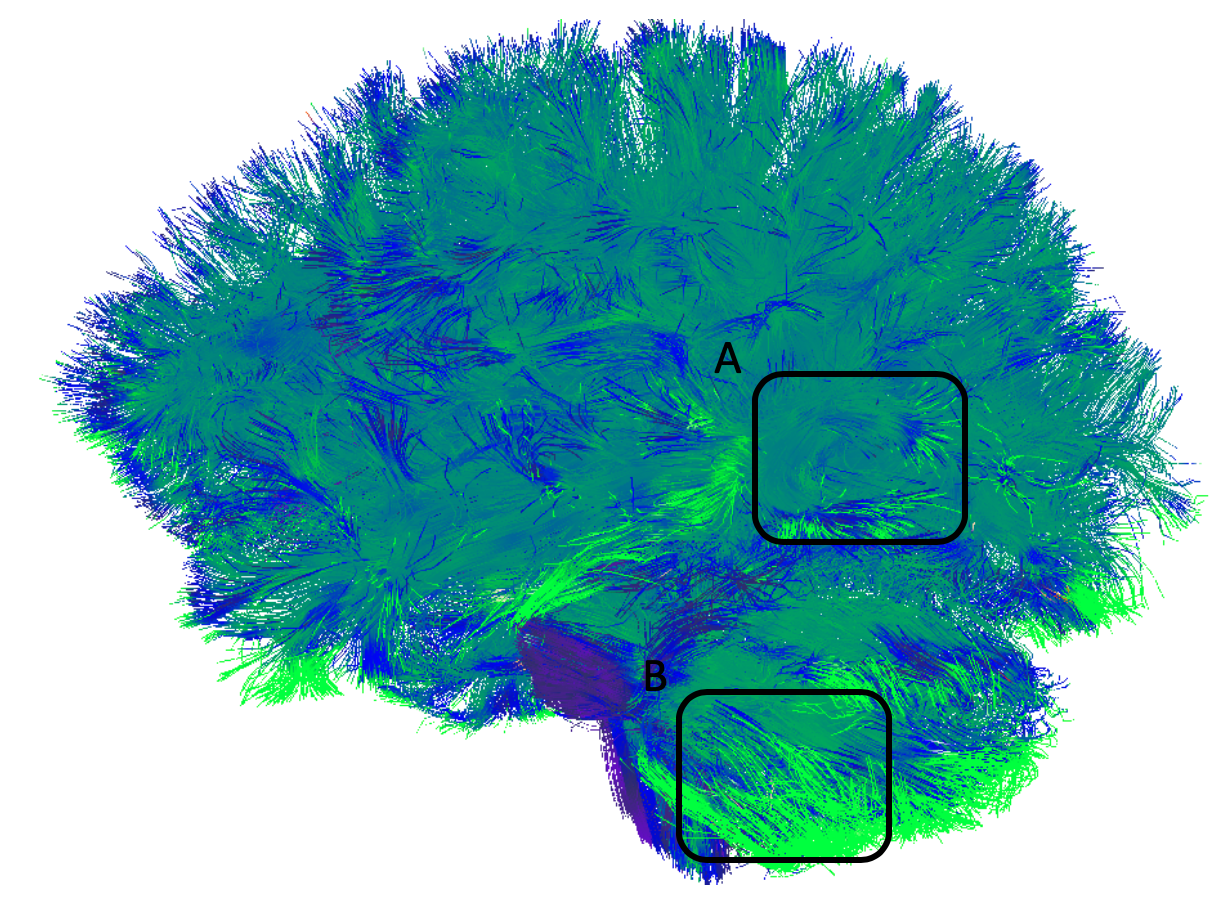
\includegraphics[width=0.8\columnwidth]{isorainbow-md-task2}
	\caption{Illustration of the questions for left side of the brain, based on Task2 for Isoluminant-rainbow colormap. top:Fa and buttom:MD}
	\label{fig:task2}
\end{figure}

	
	
Please note that Task 2 is basically the same as Task 1. However, Task 1 asks for estimate of the absolute average value  while Task 2 asks for estimate of the relation between two averages. Task 2 is clearly closer to intuition. Considerable difference in the statistical information gathered from these two tasks could lead to important conclusions.
	
\end{itemize}


\paragraph{B. Ensemble orientation}

\begin{itemize}
\item{Task 3:} The base question is: ``Follow the tracts and solve the puzzle."
This task is designed to determine which spherical colormap is better in detecting tracts and effect of color mapping on visibility of the tracts. In this task, we took a number of random zoomed pictures from two spherical colormaps of the same region of the brain. see Figure~\ref{fig:absolute-zoomed}.

\begin{figure}[ht]
    \centering
    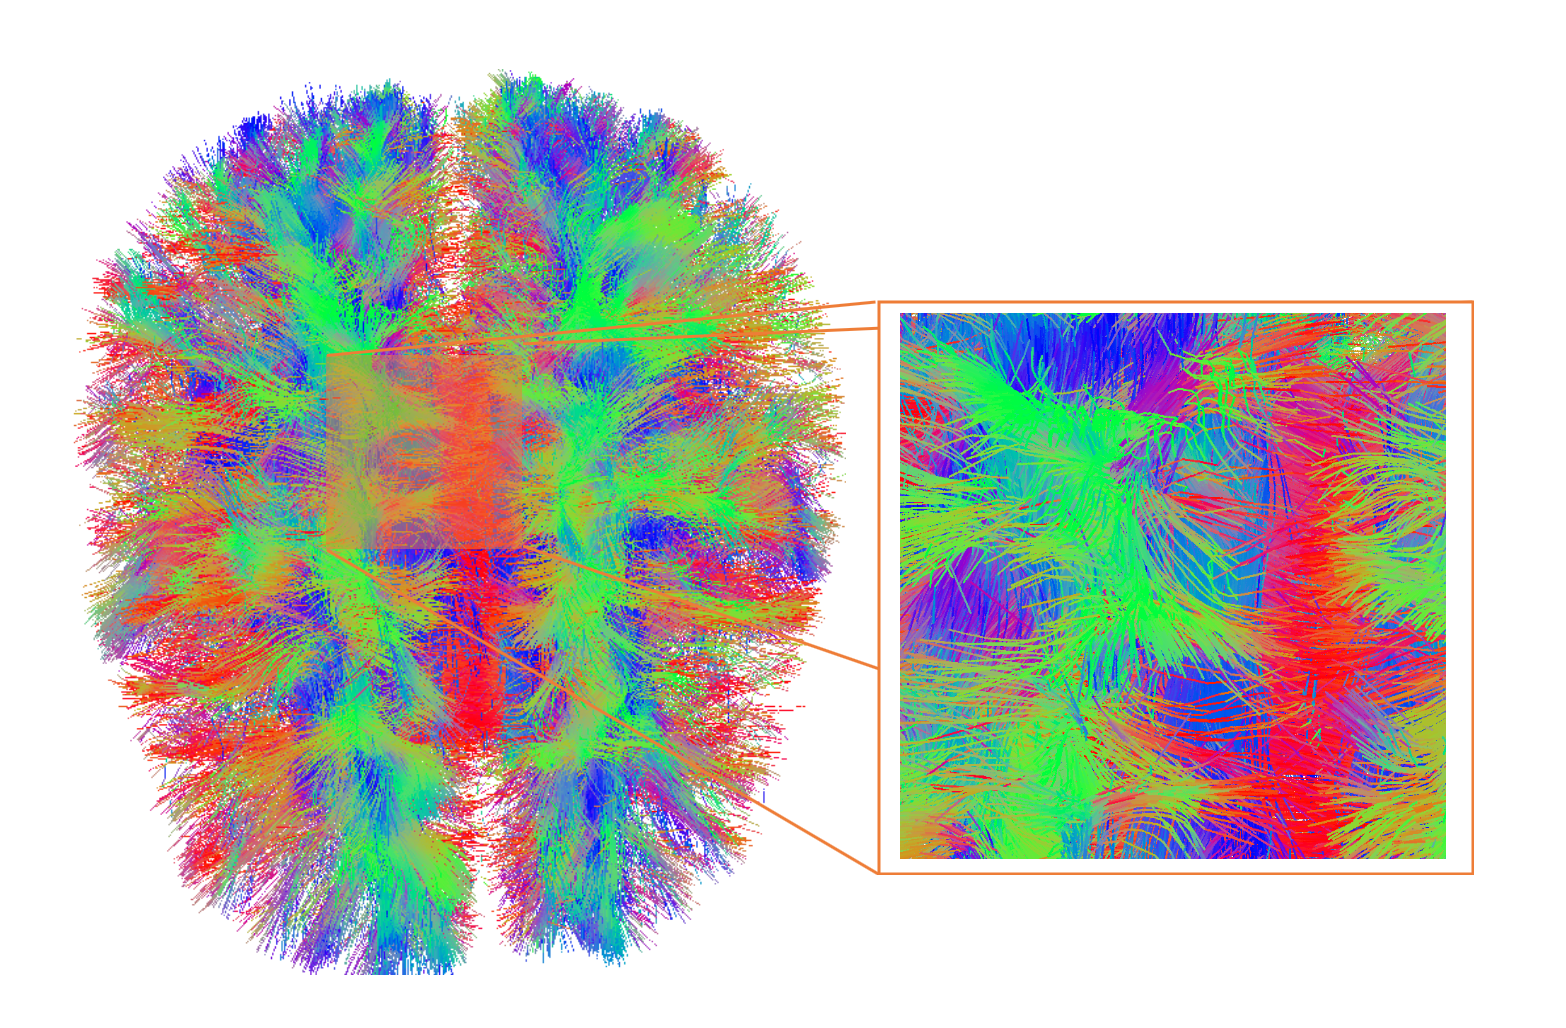
\includegraphics[width = 0.49 \columnwidth]{absolute-zoomed}
    \includegraphics[width = 0.45 \columnwidth]{boy's-zoomed}
    \caption{Zoomed random pictures of the same region of the brain for Task 3. Left:  Absolute value colormap. Right: Boy's surface colormap.}
    \label{fig:absolute-zoomed}
\end{figure}

Then the pictures were divided into nine parts like a puzzle. For guidance, a yellow/black dot is placed in the upper left corner of the image and the participants were told to firstly place this piece at the top left corner of the puzzle. see Figure~\ref{fig:absolute-puzzle}. The users are asked to solve the puzzles by following the tracts as fast as they can. The duration is recorded. 

\begin{figure}[ht]
    \centering
    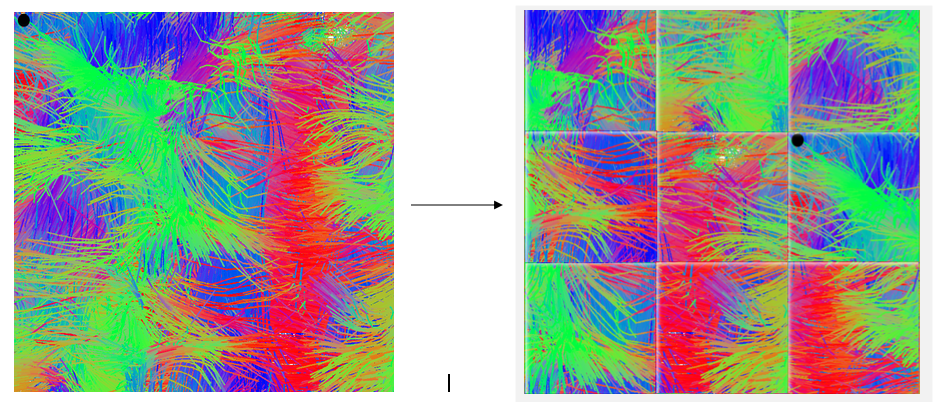
\includegraphics[width = 0.49 \columnwidth]{absolute-puzzle}
    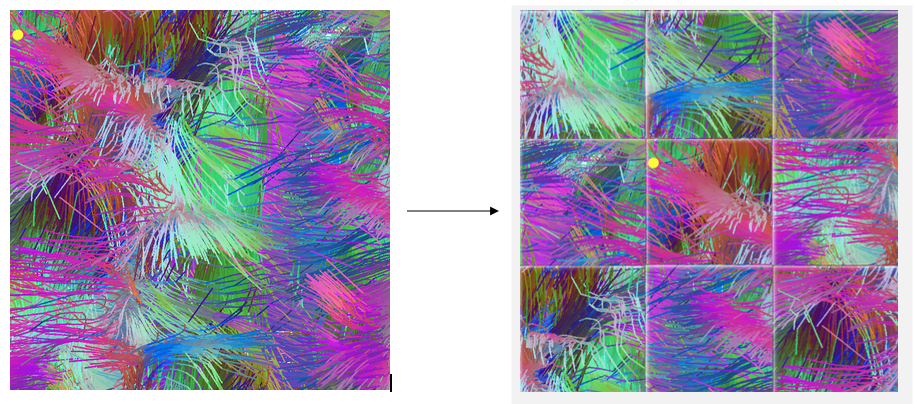
\includegraphics[width = 0.48 \columnwidth]{boy's-puzzle}
    \caption{ Samples of the puzzle for Task 3. Left:  Absolute value puzzle, Right: Boy's surface puzzle}
    \label{fig:absolute-puzzle}
\end{figure}

The statistical information should reveal which color map leads to faster identification of the orientation of the tracts. This task is designed in this particular to avoid the need for the user to interact with a GUI. This firstly removes the need for real-time rendering and makes the questionnaire available with less hardware and software requirements and secondly eliminates the role of users familiarity with complex GUIs.


\end{itemize}

\section{Procedure}
\label{procedure}
All participants first tested for normal vision with the Ishihara Color vision test. This test is online and is well-known as the Color Blind test and it is the most widely used color vision test all around the world. There are some numbers surrounded with dots and the user should distinguish the numbers out of the dots (Figure~\ref{fig:Ishihara}). If the person can get the normal color vision score it means that the user can see up to one million distinct shades of color.
\begin{figure}[ht]
    \centering
    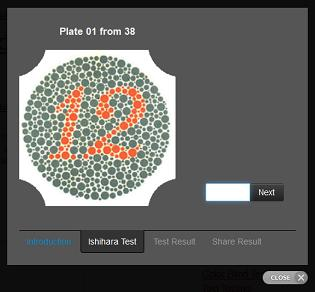
\includegraphics[width = 0.6\columnwidth]{Ishihara}
    \caption{Ishihara color blindness test. Source:  \cite{www.color-blindness.com}}
    \label{fig:Ishihara}
\end{figure}

For understanding the tasks each participants received general information about the test structure, DMRI techniques and their medical applications. These information took about 10 minutes. 

All participants were told to finish the test as soon as possible. But they could take a break at anytime. The questionnaire time was started when the user started the test until the final task was answered. 
All of them examined all colormaps.

\section{Results}
\subsection{Practical considerations }
\paragraph{Particpants} In our study, we selected 15 participants (7 male and 8 female). The  mean age was 30.5 years with standard deviation of 3 years. Their majors were: 4 medical students, 5 computer science PhD and Master students, and 6 from other disciplines (PhD and Master student in Communication Engineering, Management and sport science). All participants had normal vision by Ishihara color blindness test test as explained in Section \ref{procedure}. The cooperation of the participants was completely voluntary.

\paragraph{Hardware and Software} The program ran on a computer with 13.3-inch (diagonal) LED-backlit display with IPS technology, 2560-by-1600 native resolution at 227 pixels per inch. As there was no interaction between the user and the GUI, i.e. no real-time rendering, the specification of the CPU, GPU and operating system is not mentioned. 

\paragraph{Implementation of Tasks} The following practical limitations were taken into account in carrying out the user study:
\begin{itemize}
	\item Participation was voluntary so considerable effort from the participant's side could not be expected.
	\item Interactive GUI would require suitable hardware and software which was not available to all members of the team.
	\item Some questions require manipulation of the tractography data and insertion of 3D objects into the final rendering which was beyond the resources of the work.
\end{itemize}
As a conclusion, Task 3 was chosen for the actual questionnaire, which as described before does not conflict with the above constraints.

\subsection{Data}

The data collected for Task 3 was 
\begin{itemize}
	\item Duration: the amount of time it took for the user to finish the puzzle.
	\item Number of steps: the number of swaps done by the participant to finish the puzzle.
\end{itemize}
The users were asked to solve the puzzle by following the tracts instead of trial and error. However, not all followed this requirement. The resulting data points were therefore left out. The original data is gathered is shown in Figure~\ref{fig:rawData}.

\bibliography{biblio}
\bibliographystyle{plain}

\end{document}
